% !TeX root = presentation.tex
% !TeX program = xelatex
% ============================================================
%  Potential-Based Reward Shaping for Planar Pushing
%  Single-Agent Control vs Asymmetric Self-Play
%  Master Thesis Presentation — 30 minutes, 16:9
%  Theme: SimplePlusAIC (requires XeLaTeX or LuaLaTeX)
% ============================================================
\PassOptionsToPackage{table,dvipsnames}{xcolor}
\documentclass[aspectratio=169,xcolor=dvipsnames,t]{beamer}
\usepackage{fontspec}  % REQUIRED before theme for Epilogue font
\usepackage{colortbl}  % required for \rowcolor in tables
\usetheme{SimplePlusAIC}

\usepackage{amsmath,amssymb,amsfonts}
\usepackage{bm}
\usepackage{graphicx}
\usepackage{booktabs}
\usepackage{multirow}
\usepackage{tikz}
\usetikzlibrary{positioning,arrows.meta}
\usepackage{hyperref}

% --- Override AIC logo (not applicable to University of Groningen) ---
\logo{}

% --- Fix slide numbering (theme's /total breaks with [plain] frames) ---
\setbeamertemplate{footline}{%
  \begin{beamercolorbox}[ht=3em,sep=0.75em,wd=\paperwidth,leftskip=0.5cm,rightskip=0.5cm]{footlinecolor}
    \scriptsize{\insertshortinstitute}
    \hfill
    \scriptsize{\insertframenumber}
  \end{beamercolorbox}%
}

% --- Custom colors (complementary to theme's Bordeaux/DarkBordeaux/Astronaut) ---
\definecolor{hlblue}{RGB}{0,102,204}
\definecolor{hlgreen}{RGB}{0,140,60}
\definecolor{hlred}{RGB}{190,30,30}
\definecolor{lightgray}{RGB}{220,220,220}

% --- Literature footer ---
\newcommand{\litfooter}[1]{%
  \vspace{2pt}%
  \hrule%
  \vspace{2pt}%
  {\tiny\color{LightDarkGrey} #1}%
}

% --- Full-bleed image frame (plain, no title/footer) ---
\newcommand{\fullbleedframe}[1]{%
  \begin{frame}[plain]
    \centering
    \includegraphics[width=\paperwidth,height=\paperheight,keepaspectratio]{#1}%
  \end{frame}%
}

% --- Media box: show image if present, else a labeled placeholder ---
% #1 = width fraction of \textwidth, #2 = file name in figures/
\newcommand{\mediabox}[2]{%
  \IfFileExists{figures/#2}{%
    \includegraphics[width=#1\textwidth]{figures/#2}%
  }{%
    \setlength{\fboxsep}{6pt}%
    \fcolorbox{LightDarkGrey}{lightgray}{%
      \begin{minipage}[c][0.26\textheight][c]{#1\textwidth}%
        \centering\small\itshape [clip placeholder]\\[3pt]
        \texttt{\footnotesize \detokenize{figures/#2}}\\[3pt]record \& drop file here%
      \end{minipage}%
    }%
  }%
}

% --- Clickable "play clip" link (works in Okular / Adobe via run:) ---
\newcommand{\playclip}[1]{\href{run:figures/#1}{\scriptsize\color{hlblue}$\blacktriangleright$ play clip}}

% --- Title info ---
\title[PBRS for Planar Pushing]{Potential-Based Reward Shaping \\for Planar Pushing}
\subtitle{Single-Agent Control vs.\ Asymmetric Self-Play}
\author{Vlad Iftime s3426394}
\institute[University of Groningen, FSE]{Faculty of Science and Engineering, Artificial Intelligence \\ University of Groningen}
\date{June 2026}

% --- Final page text ---
\finalpagetext{Thank You — Questions?}

\begin{document}

% ============================================================
% TITLE PAGE (theme macro)
% ============================================================
\addtobeamertemplate{title page}{\vspace{-14pt}}{}
\maketitlepage

% ~~~~~ SPEAKER NOTES ~~~~~
\note[itemize]{
\item Welcome — 30-minute presentation on my master thesis
\item Topic: using potential-based reward shaping to train a UR5e robot arm to push objects to goal poses
\item I built 8 model variants and systematically compared them
\item Key finding: the simplest model wins — PBRS single-agent achieves 80\% validation success
\item Adding curriculum or self-play does not improve performance — every complexity degrades results
\item I'll explain why and what this means for RL in contact-rich manipulation
}

% ============================================================
% SLIDE 0 — OVERVIEW
% ============================================================
\begin{frame}[t]{Overview — Thesis Structure}
  \vspace*{-0.35cm}
  \footnotesize
  \begin{columns}[T,onlytextwidth]
    \begin{column}{0.24\textwidth}
      {\textbf{\color{hlblue}1.\ \ The Problem}}
      \begin{itemize}
        \item MDP Formulation
        \item Push Mechanics \\ (Limit Surface)
        \item Old Ad-hoc Reward \\ Failure
      \end{itemize}
    \end{column}
    \begin{column}{0.24\textwidth}
      {\textbf{\color{hlblue}2.\ \ PBRS Solution}}
      \begin{itemize}
        \item PBRS Theory
        \item Potential Functions
        \item SE(2) Unified \\ Distance Metric
      \end{itemize}
    \end{column}
    \begin{column}{0.24\textwidth}
      {\textbf{\color{hlblue}3.\ \ What We Built}}
      \begin{itemize}
        \item \textbf{A}: PBRS Single-Agent
        \item \textbf{B}: Forced Curriculum
        \item \textbf{C–D}: ASP (Alice/Bob)
        \item \textbf{E–H}: ASP Variants \\ (SE(2), disc, time-based)
      \end{itemize}
    \end{column}
    \begin{column}{0.24\textwidth}
      {\textbf{\color{hlgreen}4.\ \ What We Found}}
      \begin{itemize}
        \item PBRS outperforms \\ ad-hoc reward
        \item ASP severely \\ underperforms
        \item Reward and curriculum \\ are independent
        \item Simplest model wins \\ every time
      \end{itemize}
    \end{column}
  \end{columns}
\end{frame}

% ~~~~~ SPEAKER NOTES ~~~~~
\note[itemize]{
\item This is the roadmap for the whole talk — four stages, left to right
\item Stage 1, Planar Pushing MDP: I define the task, the quasi-static push mechanics (limit surface), and the SE(2) distance metric
\item Stage 2, PBRS Theory: why the old ad-hoc reward failed, then the potential-based reward shaping theory and our potential functions
\item Stage 3, 8 Model Variants: Model A (PBRS single-agent, our best), Model B (curriculum), and Models C–H (asymmetric self-play)
\item Stage 4, Key Findings: why ASP fails, the central independence result, computational overhead, and the overall comparison and conclusions
\item Next slide states the three research questions that this roadmap answers
}

% ============================================================
% SLIDE 1 — RESEARCH QUESTIONS
% ============================================================
\begin{frame}[t]{Research Questions}
  \begin{block}{Three Research Questions}
    \begin{enumerate}
      \item \textbf{RQ1:} Can potential-based reward shaping replace hand-tuned dense rewards for planar pushing tasks?
      \item \textbf{RQ2:} Does curriculum learning or asymmetric self-play improve sample efficiency over a direct single-agent approach?
      \item \textbf{RQ3:} Are reward design and curriculum design \emph{independent} problems in contact-rich manipulation?
    \end{enumerate}
  \end{block}

  \vspace{2pt}
  \vfill\litfooter{[Ng, Harada \& Russell 1999]~\textbf{[Grze\'s 2017]}~[Devlin \& Kudenko 2012]}
\end{frame}

% ~~~~~ SPEAKER NOTES ~~~~~
\note[itemize]{
\item RQ1: Yes — Model A achieves 80\% validation SR on 30 held-out T-block scenes
\item RQ2: No — curriculum (Model B, 76.7\%) and ASP (Models C-H, 6.7–16.7\%) both underperform the simple single-agent
\item RQ3: Yes — and this is the central contribution. The 2$\times$2 ablation shows they are independent levers
\item Roadmap: I'll define the MDP, explain why PBRS was needed, walk through each model, and present the comparison
\item 8 models, ~3000 iterations each, 528 parallel environments on an RTX Pro 6000
}

% ============================================================
% SLIDE 2 — MDP FORMULATION
% ============================================================
\begin{frame}[t]{MDP Formulation — State \& Action}
  \begin{columns}[T]
    \begin{column}{0.58\textwidth}
      \textbf{State} $\mathbf{s} \in \mathbb{R}^{28}$: \\[2pt]
      {\small $\mathbf{s} = [\;\underbrace{\mathbf{q}_{\text{ee}}}_{\text{EE pose}(6)}\;|\;
        \underbrace{\mathbf{p}_{\text{obj}}, \mathbf{R}_{\text{obj}}}_{\text{obj state}(14)}\;|\;
        \underbrace{\mathbf{p}_{\text{goal}}, \mathbf{R}_{\text{goal}}}_{\text{goal pose}(6)}\;|\;
        \underbrace{d_{\text{pos}}, d_{\text{rot}}}_{\text{errors}(2)}\;]$}

      \vspace{4pt}
      \textbf{Action} $\mathbf{a} \in \mathbb{R}^4$ (object-relative): \\[2pt]
      {\small $(r,\phi,\ell,\theta)$ with 21 bins/dim $\Rightarrow$ 194\,481 discrete actions}
      \[
      \begin{aligned}
      X_s &= x_{\text{obj}} + r \cos(\psi_{\text{obj}} + \phi) \\
      Y_s &= y_{\text{obj}} + r \sin(\psi_{\text{obj}} + \phi) \\
      X_f &= X_s + \ell \cos\theta,\quad Y_f = Y_s + \ell \sin\theta
      \end{aligned}
      \]
    \end{column}
    \begin{column}{0.38\textwidth}
      \centering
      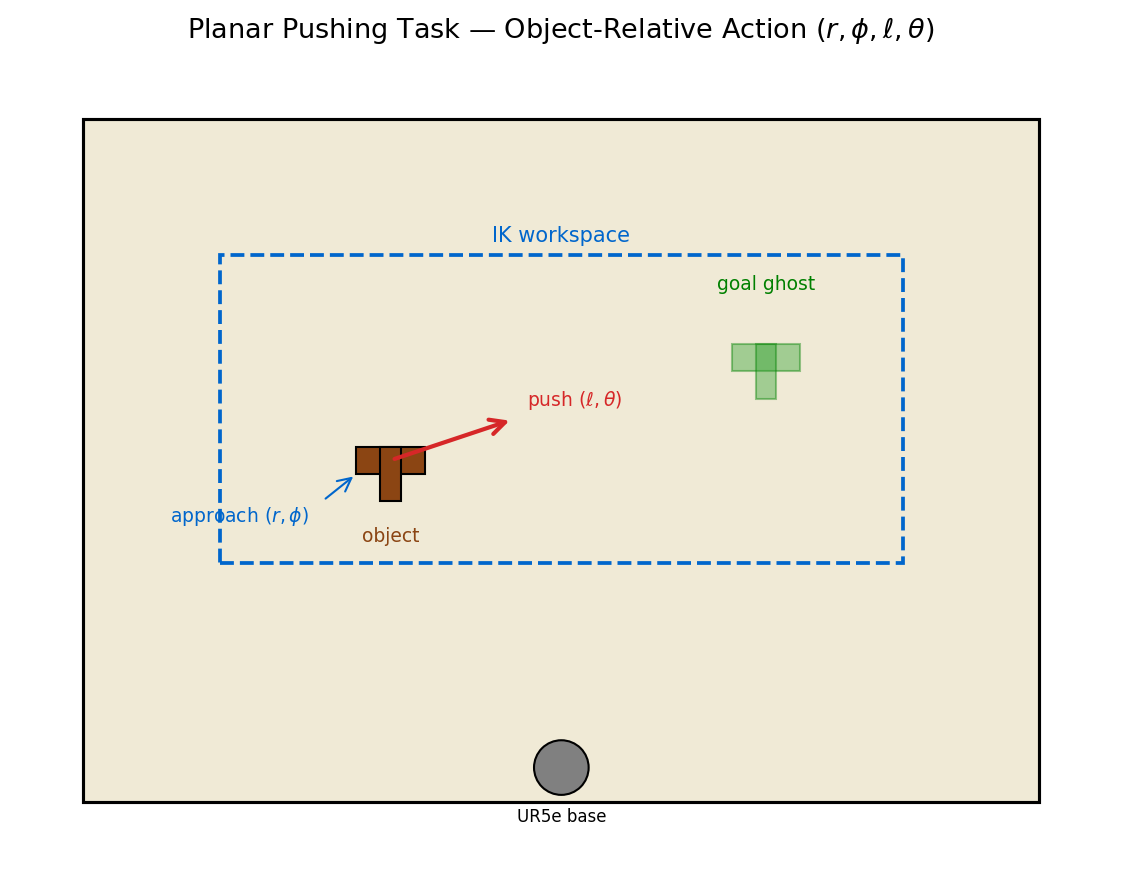
\includegraphics[width=1.0\textwidth]{figures/diagram_task_schematic.png}
      \vspace{2pt}
    \end{column}
  \end{columns}

  \vfill\litfooter{[Mason 1986]~[Lynch \& Mason 1996]~[Goyal et al.\ 1991]}
\end{frame}

% ~~~~~ SPEAKER NOTES ~~~~~
\note[itemize]{
\item The MDP is a planar pushing task: a UR5e robot pushes a T-block or disc object on a 1.4m × 1.0m table
\item State is 28D: end-effector pose (6), object state including position and quaternion (14), goal pose (6), and current distance errors (2)
\item Action is 4D macro-parameterized as object-relative approach (r, phi) plus world-frame push direction (length, theta). 21 bins per dimension = 194k discrete actions
\item Object-relative actions are critical — they guarantee ~95\% contact rate regardless of object spawn position, vs ~2\% for absolute coordinates
}

% ============================================================
% SLIDE 2b — MDP: TRANSITION & EPISODE
% ============================================================
\begin{frame}[t]{MDP Formulation — Transition \& Episode}
  \begin{columns}[T,onlytextwidth]
    \begin{column}{0.56\textwidth}\small
      \textbf{Transition — quasi-static limit surface} (Mason 1986): $\mathbf{t} = (v_x, v_y, \omega) \propto \nabla f(\mathbf{w})$. Object twist is normal to the surface — every push couples translation \emph{and} rotation.

      \vspace{3pt}
      \textbf{Episode:}
      \begin{itemize}
        \item Max 15 pushes (training); validation uses 30 pushes, best-of-20 retries
        \item Success $=$ pos $<$ 5\,cm \textbf{and} rot $<$ 0.2\,rad
        \item Ends early on catastrophe (tipped / launched / OOB)
        \item Table $1.40\times1.00$\,m; IK $X\!\in\![-0.5,0.5]$, $Y\!\in\![0.25,0.70]$\,m
      \end{itemize}
    \end{column}
    % \begin{column}{0.42\textwidth}
    %   \centering
    %   \mediabox{1.0}{gif_push_sequence_key.png}\\[2pt]
    %   {\scriptsize Push sequence (start\,$\to$\,3 pushes\,$\to$\,goal)}\quad\playclip{gif_push_sequence.gif}
    % \end{column}
  \end{columns}

  \vfill\litfooter{[Mason 1986]~[Lynch \& Mason 1996]~[Goyal et al.\ 1991]}
\end{frame}

% ~~~~~ SPEAKER NOTES ~~~~~
\note[itemize]{
\item The physics is quasi-static: the object motion is determined by the limit surface normality theorem — every push couples translation and rotation
\item Episode runs max 15 pushes. Terminates on combined success (pos < 5cm AND rot < 0.2 rad) or on catastrophe (tipped, launched, out-of-workspace)
\item The table is 1.40m × 1.00m, IK workspace X ∈ [−0.50, 0.50], Y ∈ [0.25, 0.70]
\item GIF suggestion shows a real robot doing 3 pushes to reach a goal — this grounds the abstract MDP in the physical task
}
% Slide 3a moved to appendix (Push Mechanics — Limit Surface + L)
% ============================================================


% ============================================================
% SLIDE 3b — SE(2) UNIFIED DISTANCE
% ============================================================
\begin{frame}[t]{SE(2) Unified Distance — Models E-H}
  \begin{columns}[T,onlytextwidth]
    \begin{column}{0.54\textwidth}
      \textbf{SE(2) metric:} $d_{\text{pose}} = \sqrt{dx^2 + dy^2 + L^2 d\theta^2}$
      \begin{itemize}
        \item Single scalar combining $(dx,dy)$ and $d\theta$; $L$ = char.\ length (T-block $0.07$m, disc $0$m)
        \item \textbf{Single-potential PBRS:} $\Phi(s)=w\,e^{-k\,d_{\text{pose}}^2}$, $k=30,\,w=10$
        \item Eliminates competing pos/rot gradients — aligns reward with the coupled physics
      \end{itemize}
      \textbf{Result:} SE(2) does \emph{not} rescue ASP — E/F reach only 6.7\% validation SR vs single-agent 80\%. The self-play curriculum is the root cause, not the metric.
    \end{column}
    \begin{column}{0.44\textwidth}
      \centering
      
\includegraphics[width=1.0\textwidth]{figures/diagram_limit_surface.png}
    \end{column}
  \end{columns}

  \vfill\litfooter{[Park 1995]~[Urain et al.\ 2023]~[Lynch \& Mason 1996]}
\end{frame}

% ~~~~~ SPEAKER NOTES ~~~~~
\note[itemize]{
\item The SE(2) unified distance replaces separate position and rotation errors with a single Riemannian metric on the planar rigid-body configuration space
\item L converts radians to meters. For the T-block with L=0.07m, 0.5 rad of rotation contributes 3.5cm to d_pose — roughly equal weight with a 3.5cm position displacement
\item For the disc with L=0m, rotation is irrelevant — d_pose collapses to pure position distance, matching the physical symmetry
\item The single-potential PBRS eliminates the competing gradient problem: separate pos/rot potentials each pull in different directions, while the SE(2) potential provides a unified gradient
\item Both Model E (SE(2) d_pose ASP) and Model C (separate ASP) collapse — the SE(2) metric doesn't rescue the self-play dynamics, confirming the curriculum is the root cause, not the reward metric
}

% ============================================================
% SLIDE 4 — OLD REWARD FORMULA FAILURE
% ============================================================
\begin{frame}[t]{Old Reward Formula — Why It Failed}
  \begin{block}{Fractional Improvement Formula (Fixes P63-P64)}
    \[
    R = \underbrace{\alpha\!\cdot\!\frac{d_{\text{prev}}\!-\!d_{\text{now}}}{d_{\text{prev}}}}_{\text{position improvement}}
        + \underbrace{\alpha\!\cdot\!\frac{y_{\text{prev}}\!-\!y_{\text{now}}}{y_{\text{prev}}}}_{\text{rotation improvement}}
        - \underbrace{\beta_{\text{pos}}\!\cdot\!d_{\text{now}}}_{\text{position penalty}}
        - \underbrace{\beta_{\text{rot}}\!\cdot\!y_{\text{now}}}_{\text{rotation penalty}}
    \]
    {\small $\alpha=3.0,\;\beta_{\text{pos}}=0.5,\;\beta_{\text{rot}}=0.25$\\
    $d_{\text{prev}},d_{\text{now}}$: position error before/after push;\; $y_{\text{prev}},y_{\text{now}}$: rotation error before/after push}
  \end{block}

  \vspace{-6pt}
  \begin{columns}[T]
    \begin{column}{0.50\textwidth}
      {\footnotesize \textbf{Problem 1 — Non-Markov:} Depends on $d_{\text{prev}}$ — same state transition gets different reward from different starting positions. Value function ill-defined.}
    \end{column}
    \begin{column}{0.46\textwidth}
      {\footnotesize \textbf{Problem 2 — Gradient Starvation:} 1cm improvement from 30cm: \textcolor{hlred}{$\alpha\!\cdot\!0.01/0.30 - \beta_{\text{pos}}\!\cdot\!0.29 = \mathbf{-0.045}$}. Progress gets $\mathbf{negative}$ reward. $\mathbb{E}[R] \approx -0.15$, near-zero variance.}
    \end{column}
  \end{columns}

  \vspace{-2pt}
  {\footnotesize \textbf{Result:} The fractional formula suffers from two structural flaws — non-Markov dependence and gradient starvation — making it fundamentally unsuitable for stable RL training.}

  \vfill\litfooter{[Ng et al.\ 1999]~[Grzes \& Kudenko 2009]}
\end{frame}

% ~~~~~ SPEAKER NOTES ~~~~~
\note[itemize]{
\item The old fractional improvement formula had two fatal flaws
\item First, it's non-Markov: dividing by d_prev makes reward depend on starting position. The same state transition gets different reward. I prove in my thesis appendix that no static potential Phi(s) can reproduce this reward
\item Second, gradient starvation: a push producing genuine progress gets penalized because the penalty term dominates. The expected reward for random pushes is negative with near-zero variance — PPO's GAE gets no signal to differentiate good from bad pushes
\item This is WHY we needed a better reward function — PBRS fixes both problems
}

% ============================================================
% SLIDE 5a — PBRS THEOREM
% ============================================================
\begin{frame}[t]{PBRS — Why It's the Right Choice}
  \textbf{Ng et al.\ (1999) Shaping Theorem:}
  \[
  \boxed{\mathcal{R}'(s,a,s') = \mathcal{R}(s,a,s') + \underbrace{\gamma\Phi(s') - \Phi(s)}_{\text{shaping reward }F}}
  \]
  \begin{itemize}
    \item $\mathcal{R}$ — original (true/sparse) reward; $\mathcal{R}'$ — shaped reward the agent sees
    \item $\Phi(s)$ — any scalar function of state (the \emph{potential}); $\gamma$ — MDP discount
    \item \textbf{Policy invariance:} $Q'(s,a) = Q(s,a) - \Phi(s)$ — optimal actions unchanged
  \end{itemize}

  \textbf{Our potential functions (Models A/B):}
  \[
  \Phi(s) = w_{\text{pos}} e^{-k_p d_{\text{pos}}^2} + w_{\text{rot}} e^{-k_r c(s)},\quad
  c(s) = \frac{1-\cos(\theta^*-\theta)}{2}
  \]
  $k_p{=}30,\; k_r{=}5,\; w_{\text{pos}}{=}w_{\text{rot}}{=}10.0$\quad
  \textbf{Dense reward:} $F(s,s') = \Phi(s') - \Phi(s)$

  \textbf{Why ideal for planar pushing:}
  \begin{enumerate}
    \item \textbf{Markovian} — depends only on $s,s'$; \textbf{Bounded} — exponentials prevent PhysX spikes
    \item \textbf{Zero-sum cycles} — detour pushes net to zero; \textbf{No constant drain} — $F{=}0$ when stationary
    \item \textbf{Episodic PBRS} (Grze\'s 2017): $\gamma_{\text{shaping}}{=}1.0$ valid — $\sum F = \Phi(s_T)-\Phi(s_0)$ bounded
  \end{enumerate}

  \vfill\litfooter{[Ng, Harada \& Russell 1999]~\textbf{[Grze\'s 2017]}~[Devlin \& Kudenko 2012]}
\end{frame}

% ~~~~~ SPEAKER NOTES ~~~~~
\note[itemize]{
\item The fundamental theorem: add F = gamma·Phi(s') − Phi(s) without changing the set of optimal policies
\item Proof: Q'(s,a) = Q(s,a) − Phi(s). Since Phi(s) depends only on state (not action), the argmax is unchanged
\item Our potential: sum of two exponentiated distance functions for position and rotation
\item Cosine distance c(s) respects S¹ topology — no discontinuity at ±π
\item Episodic PBRS (Grześ 2017): gamma_shaping=1.0 is valid because the sum over an episode is bounded
\item Six key properties: policy invariance, Markovian, bounded, zero-sum cycles, no constant drain, natural gradient toward goal
}

% ============================================================
% SLIDE 5b-ii — PBRS REWARD DIET
% ============================================================
\begin{frame}[t]{Why PBRS Works — The Reward Diet}
  {\small\textbf{Reward composition:}
  \begin{itemize}
    \item Dense PBRS shaping $\approx$85\% of reward — a signal on \emph{every} push
    \item Sparse bonuses ($+5$/$+2$) and catastrophe penalties are supplementary; bounded potentials keep it stable
  \end{itemize}}

  \vspace{2pt}
  \begin{center}
    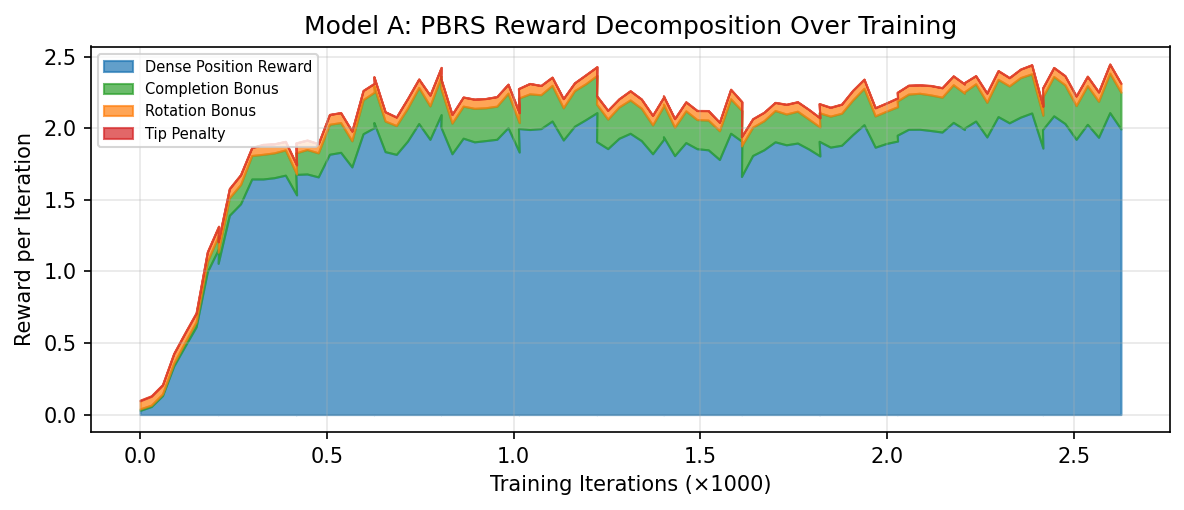
\includegraphics[width=0.50\textwidth]{figures/plot5_reward_diet.png}
  \end{center}

  \vfill\litfooter{[Ng, Harada \& Russell 1999]~\textbf{[Grze\'s 2017]}~[Harutyunyan et al.\ 2015]}
\end{frame}

% ~~~~~ SPEAKER NOTES ~~~~~
\note[itemize]{
\item The reward diet plot shows the agent gets ~85\% of its reward from dense PBRS shaping, with sparse bonuses and penalties as supplementary signals
\item Because the dense signal fires every push and is bounded, the critic stays stable and PPO always has a gradient to follow
}

% ============================================================
% SLIDE 5b-ii — PBRS POTENTIALS: WHY IT WORKS
% ============================================================
\begin{frame}[t]{PBRS — Why Our Potentials Work}
  {\small\textbf{Why this works for planar pushing:}
  \begin{itemize}
    \item Bounded exponentials $\to$ no reward explosions; $\Phi(s')-\Phi(s)$ gives a natural gradient toward the goal
    \item Cosine distance respects $\mathbb{S}^1$ topology; hyperparameters robust across 3 independent runs
  \end{itemize}}

  \vspace{2pt}
  \begin{center}
    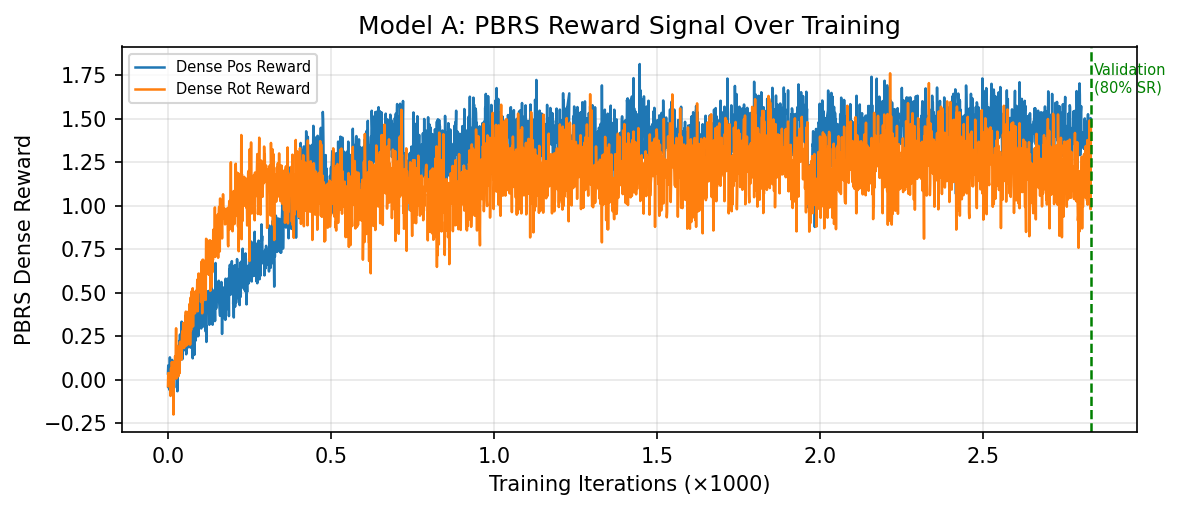
\includegraphics[width=0.50\textwidth]{figures/plot1_pbrs_signal_vs_performance.png}
  \end{center}

  \vfill\litfooter{[Ng et al.\ 1999]~[Grze\'s 2017]~[Harutyunyan et al.\ 2015]}
\end{frame}

% ~~~~~ SPEAKER NOTES ~~~~~
\note[itemize]{
\item Bounded exponential potentials prevent reward explosions from PhysX glitches; the potential difference gives a natural gradient toward the goal
\item Cosine distance respects the S^1 topology of rotation
\item These hyperparameters are robust: 3 independent training runs with identical settings all converged to similar performance
}

% ============================================================
% SLIDE 6a — MODEL A: ARCHITECTURE + TRAINING
% ============================================================
\begin{frame}[t]{Model A — PBRS Single-Agent (Our Best Model)}
  \small
  \textbf{Architecture:} Single PPO agent, LSTM(28$\to$256) + MLP[512, 256] trunk, MultiCategorical head (4 dims $\times$ 21 bins). No curriculum, no Alice/Bob, no GoalEncoder.

  \textbf{Training:} 528 envs, 15 pushes/rollout, $\sim$3000 iterations on RTX Pro 6000. $\sim$1.6 days wall-clock ($\sim$0.022 it/s).

  \textbf{Why it works:}
  \begin{enumerate}
    \item \textbf{Dense, bounded gradient} — PBRS fires on every push
    \item \textbf{Fixed goal distribution} — stationary random goals; no adversarial shift
    \item \textbf{Single network} — one agent, one optimizer; no multi-agent instability
  \end{enumerate}

  \vfill\litfooter{[Ng et al.\ 1999]~[Grze\'s 2017]~[Schulman et al.\ 2017]}
\end{frame}

% ~~~~~ SPEAKER NOTES ~~~~~
\note[itemize]{
\item Model A is the simplest possible architecture: single PPO agent with LSTM+MLP, PBRS reward, sparse completion bonuses
\item Three reasons it works: PBRS provides dense gradient at every push, fixed random goal distribution avoids adversarial shift, single network avoids multi-agent optimization instability
\item Converges within 1500 iterations. Stable value function bounded by exponential potentials
}

% ============================================================
% SLIDE 6b — MODEL A: TRAINING CURVES
% ============================================================
\begin{frame}[t]{Model A — Training Dynamics}
  \begin{center}
    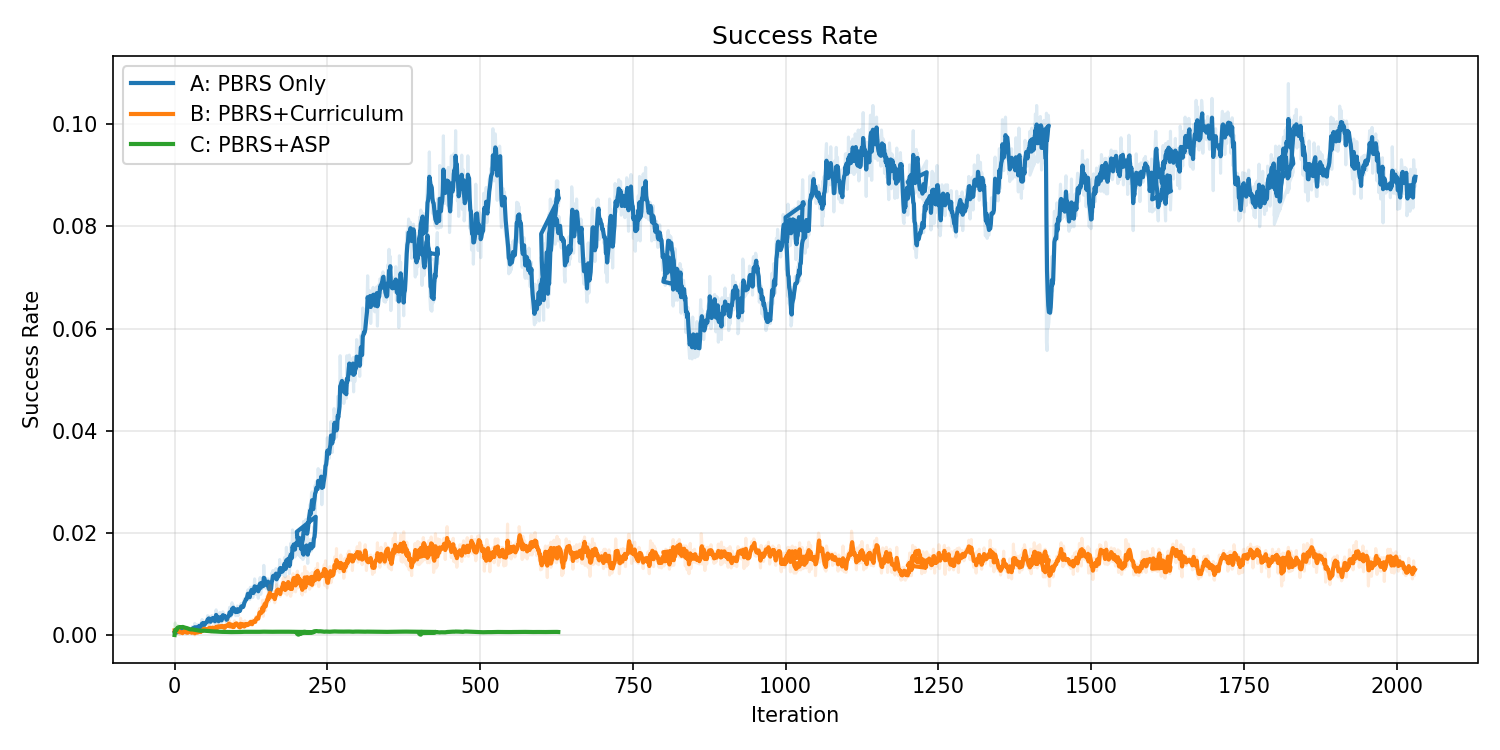
\includegraphics[width=0.50\textwidth]{figures/cmp_Success_Rate.png}
    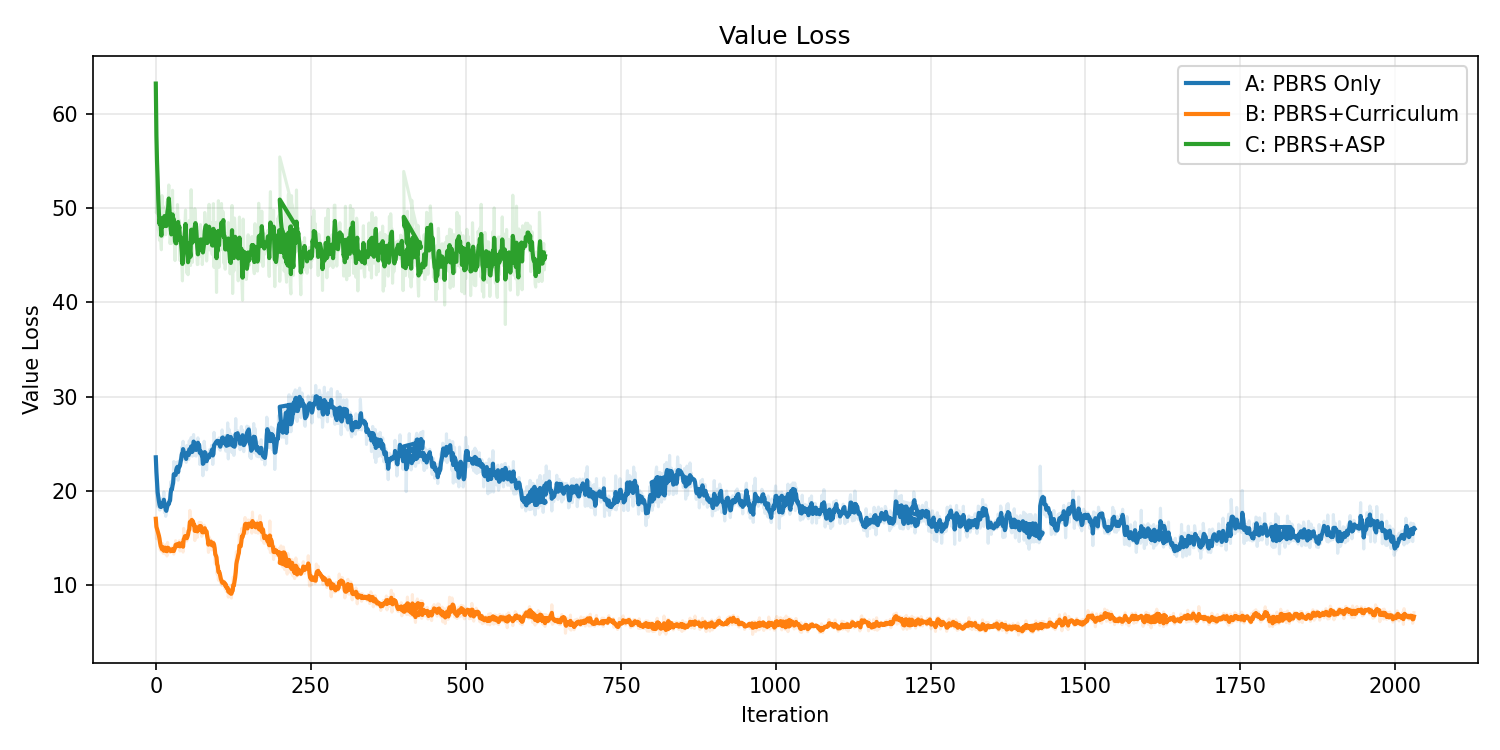
\includegraphics[width=0.50\textwidth]{figures/cmp_Value_Loss.png}
  \end{center}

  \vspace{2pt}
  {\small \textbf{Left:} Model A (blue) steadily improves training success rate over 3000 iterations. Model B (orange) follows a similar trajectory but converges slightly lower. ASP variants (E–H) remain near baseline throughout. \textbf{Right:} Stable value function — no explosion. Initial $V\approx0.057$ with gain$=0.01$.}

  \vfill\litfooter{[Schulman et al.\ 2017]~[Ng et al.\ 1999]}
\end{frame}

% ~~~~~ SPEAKER NOTES ~~~~~
\note[itemize]{
\item Left plot: training success rate over ~3000 iterations. Model A (blue) improves from near-zero to ~9.4\% (strict combined gate). Model B (orange, P82-fixed) follows a similar trajectory. ASP variants (E-H) remain near baseline
\item Right plot: value loss stays stable — no explosion. The PBRS exponential potentials prevent the reward spikes that caused GAE chain reactions and critic instability in earlier attempts
}

% ============================================================
% SLIDE 6c — MODEL A: VALIDATION RESULTS
% ============================================================
\begin{frame}[t]{Model A — Validation Results}
  \begin{columns}[T,onlytextwidth]
    \begin{column}{0.50\textwidth}
      \textbf{30 held-out T-block scenes (best-of-20):}
      \begin{itemize}
        \item \textcolor{hlgreen}{\textbf{80.0\% SR}} (24/30) — pos-only \textbf{100\%}, pos+rot \textbf{70\%}
        \item PosErr \textbf{0.032\,m}, RotErr \textbf{0.568\,rad}
        \item Training SR ($\sim$9.4\%) understates validation — strict combined gate vs best-of-20
      \end{itemize}
    \end{column}
    \begin{column}{0.48\textwidth}
      \centering
      \mediabox{1.0}{rec_push_s21_key.png}\\[2pt]
      {\scriptsize Overhead view — Model A solving a pos+rot scene}\quad\playclip{rec_push_s21.mp4}
    \end{column}
  \end{columns}

  \vfill\litfooter{[Ng et al.\ 1999]~[Grze\'s 2017]~[Schulman et al.\ 2017]}
\end{frame}

% ~~~~~ SPEAKER NOTES ~~~~~
\note[itemize]{
\item Validation: 30 held-out T-block scenes, best-of-20 protocol. 80.0\% overall SR
\item Perfect on position-only scenes (100\%), strong on combined pos+rot scenes (70\%)
\item PosErr 0.032m and RotErr 0.568 rad on successful episodes
\item Training SR (∼9.4\%) understates validation because the strict combined gate penalizes near-misses in training. Validation uses best-of-3/best-of-20 retries
\item The overhead clip shows the trained Model A policy recorded top-down
}

% ============================================================
% SLIDE 6c-i2 — MODEL A: VALIDATION RUNS (3-up overhead clips)
% ============================================================
\begin{frame}[t]{Model A — Validation Runs (overhead)}
  {\small Three held-out T-block scenes, top-down camera — the trained Model A policy:}

  \vspace{4pt}
  \begin{columns}[T,onlytextwidth]
    \begin{column}{0.32\textwidth}
      \centering
      \mediabox{1.0}{rec_push_s11_key.png}\\[2pt]
      {\scriptsize Forward (pos-only)}\quad\playclip{rec_push_s11.mp4}
    \end{column}
    \begin{column}{0.32\textwidth}
      \centering
      \mediabox{1.0}{rec_push_s13_key.png}\\[2pt]
      {\scriptsize Lateral push (pos-only)}\quad\playclip{rec_push_s13.mp4}
    \end{column}
    \begin{column}{0.32\textwidth}
      \centering
      \mediabox{1.0}{rec_push_s21_key.png}\\[2pt]
      {\scriptsize Translate + rotate}\quad\playclip{rec_push_s21.mp4}
    \end{column}
  \end{columns}

  \vfill\litfooter{[Ng et al.\ 1999]~[Grze\'s 2017]~[Schulman et al.\ 2017]}
\end{frame}

% ~~~~~ SPEAKER NOTES ~~~~~
\note[itemize]{
\item Three representative validation runs recorded top-down with record\_push\_video.py
\item Left: a short forward push (E\_Forward, position-only)
\item Middle: a lateral push (E\_Left, position-only)
\item Right: a combined translate-and-rotate scene (E\_Diag, position+rotation)
\item All use the same simple PBRS Model A checkpoint with object-relative obs+actions
}

% ============================================================
% SLIDE 6c-ii — MODEL A: VALIDATION BREAKDOWN
% ============================================================
\begin{frame}[t]{Model A — Validation Breakdown}
  \begin{columns}[T,onlytextwidth]
    \begin{column}{0.5\textwidth}
      \centering
      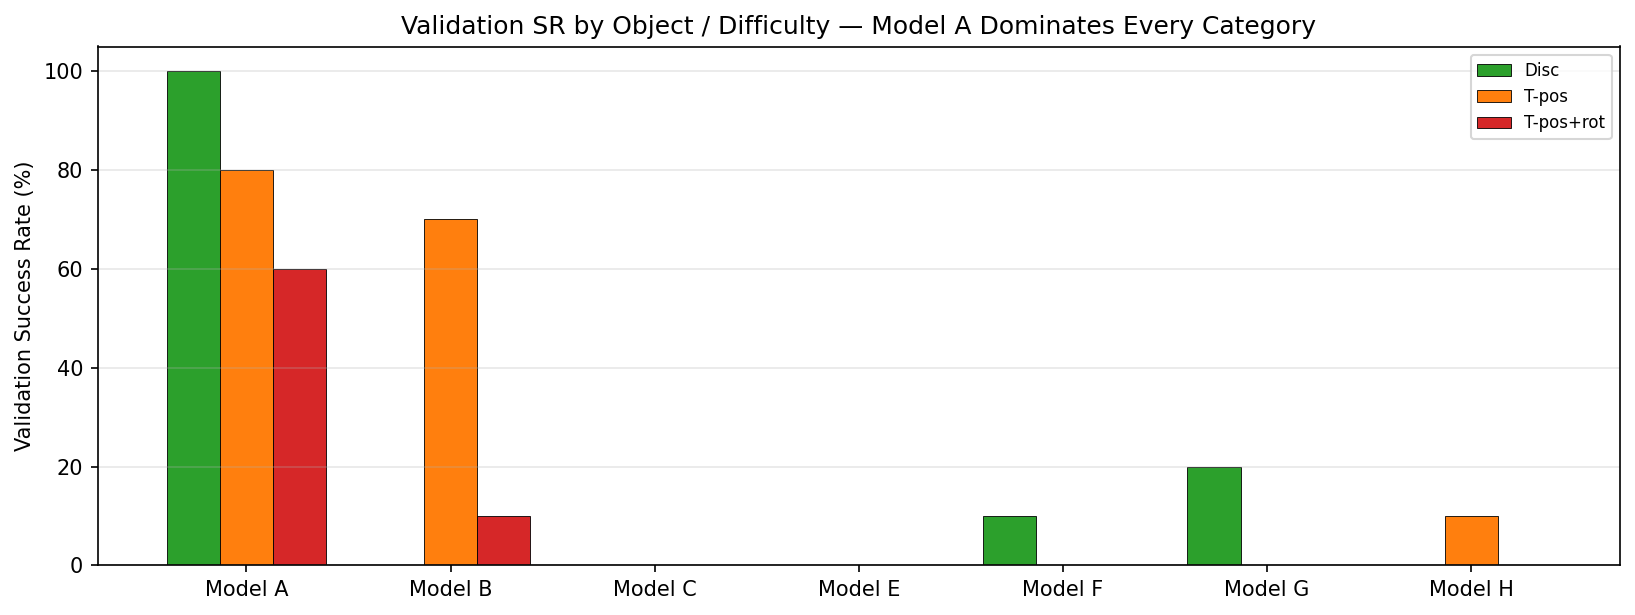
\includegraphics[width=1.0\textwidth]{figures/val_sr_bars.png}\\[2pt]
      {\scriptsize SR by difficulty — A leads all categories}
    \end{column}
    \begin{column}{0.5\textwidth}
      \centering
      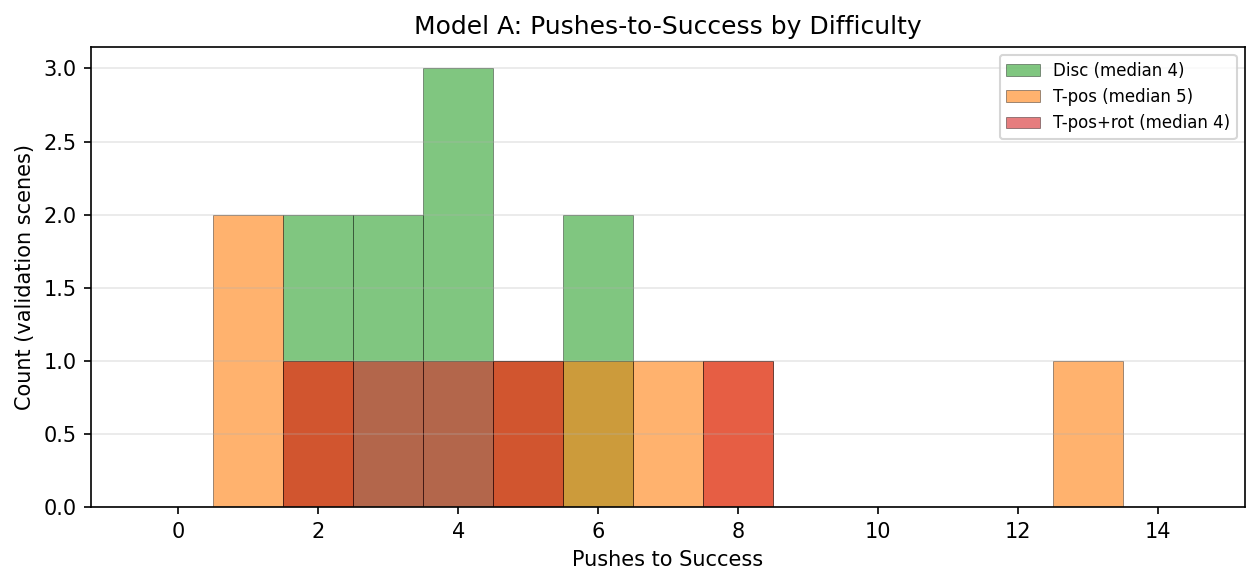
\includegraphics[width=1.0\textwidth]{figures/val_pushes_hist.png}\\[2pt]
      {\scriptsize Avg pushes per scene: easy 28.8, medium 24.2, hard 24.0}
    \end{column}
  \end{columns}

  \vfill\litfooter{[Ng et al.\ 1999]~[Grze\'s 2017]~[Schulman et al.\ 2017]}
\end{frame}

% ============================================================
% SLIDE 7 — MODEL B: FORCED CURRICULUM
% ============================================================
\begin{frame}[t]{Model B — PBRS + Forced Curriculum \hfill \textcolor{hlgreen}{(Fixed)}}
  \textbf{Design:} Same PPO agent as Model A + 3-phase curriculum:
  \begin{enumerate}
    \item $w_{\text{rot}}=0$, position-only training
    \item Triggered when episodic position-SR $\ge 0.5$ for 20 iters: $w_{\text{rot}}$ ramps $0\to10$ over 200 iters
    \item Full PBRS (multi-objective)
  \end{enumerate}

  \vspace{2pt}
  \textbf{\textcolor{hlred}{Original trigger was mis-specified:}} the first version used a per-push mean position error threshold of 0.08m — below even the \emph{best} model's validation PosErr (0.202m). The curriculum never activated because the threshold was unreachable by construction (P82 fix).

  \vspace{2pt}
  \textbf{Corrected trigger:} gates on episodic position-only SR $\ge$ 0.5 over a 20-iter lookback. Curriculum now activates and reaches \textcolor{hlgreen}{76.7\% SR} — only 3.3pp below Model A.

  \vfill\litfooter{[Narvekar et al.\ 2020]~[Portelas et al.\ 2020]~[Florensa et al.\ 2017]}
\end{frame}

% ~~~~~ SPEAKER NOTES ~~~~~
\note[itemize]{
\item Model B was designed to learn position first, then progressively add rotation — a classic curriculum approach
\item The original trigger (v1) used a per-push mean position error < 0.08m AND gate over 50 iterations. This was unreachable: even A\_simp's validation PosErr is 0.032m terminal error, but the per-push mean (across all pushes of an episode from random spawn) never drops below 0.08m because early pushes start far from a freshly randomized goal
\item With the P82 fix — episodic position-SR > 0.5 over 20 iterations — the curriculum activates. B achieves 76.7\%, only 3.3pp behind A
\item The curriculum works but doesn't beat the simpler no-curriculum baseline. The simplest model still wins
}

% ============================================================
% SLIDE 7b — MODEL B: RESULTS
% ============================================================
\begin{frame}[t]{Model B — Results: $A_{\text{simp}}$ vs $B_{\text{curr}}$}
  \begin{center}
  \footnotesize
  \begin{tabular}{lccc}
    \toprule
    \textbf{Metric} & \textbf{Model A (no curric.)} & \textbf{Model B (curriculum)} & \textbf{Gap} \\
    \midrule
    Validation SR & \textcolor{hlgreen}{\textbf{80.0\%}} & 76.7\% & 1.04$\times$ \\
    PosErr (m) & 0.032 & \textcolor{hlgreen}{\textbf{0.023}} & B 28\% lower \\
    RotErr (rad) & 0.568 & 0.663 & A 14\% lower \\
    Pos-only SR & 100\% & 100\% & equal \\
    Pos+rot SR & 70\% & 65\% & 5pp \\
    \bottomrule
  \end{tabular}
  \end{center}
  \vspace{1pt}
  {\scriptsize \textbf{Result:} Curriculum improves position precision (0.023 vs 0.032 m) from the pos-only phase, but slightly degrades rotation (0.663 vs 0.568 rad). Net effect: B is 3.3pp behind A.}
  {\scriptsize \textbf{Takeaway:} A staged curriculum \emph{can} work alongside PBRS, but does not beat the simpler no-curriculum baseline.}

  \vfill\litfooter{[Narvekar et al.\ 2020]~[Portelas et al.\ 2020]~[Florensa et al.\ 2017]}
\end{frame}

% ~~~~~ SPEAKER NOTES ~~~~~
\note[itemize]{
\item Head-to-head on identical 30 T-block scenes: A\_simp 80.0\% vs B\_curr 76.7\%
\item B actually beats A on position precision (0.023 vs 0.032 m) — the pos-only Phase 1 training produces tighter position control. But rotation is slightly worse (0.663 vs 0.568 rad)
\item Both achieve 100\% pos-only SR. The combined pos+rot gate is 70\% (A) vs 65\% (B)
\item The curriculum is functional but fails to outperform the simpler baseline. Adding structure adds complexity without adding net value
}

% ============================================================
% SLIDE 8a — ASP ARCHITECTURE
% ============================================================
\begin{frame}[t]{Models C–H — ASP Architecture (Alice/Bob)}
  \begin{columns}[T,onlytextwidth]
    \begin{column}{0.52\textwidth}
      {\small
      \textbf{Alice (Goal Proposer):}
      \begin{itemize}
        \item PPO agent, pushes object to a target pose
        \item That pose becomes Bob's goal
        \item Reward: $+5$ if Bob fails, $-1$ if Bob succeeds
      \end{itemize}

      \vspace{4pt}
      \textbf{Bob (Goal Achiever):}
      \begin{itemize}
        \item PPOABC + GoalEncoder, must reproduce Alice's goal pose
        \item Reward: PBRS dense $+$ sparse bonuses
        \item Failed trajectories $\to$ ABC buffer ($\beta_{\text{abc}}=0.5$)
      \end{itemize}}

      \vspace{4pt}
      {\small\textbf{Variants:} C (base ASP), D (no GoalEncoder), E/F (SE(2) $d_{\text{pose}}$), G/H (time-based Alice reward).}
    \end{column}
    \begin{column}{0.46\textwidth}
      \centering
      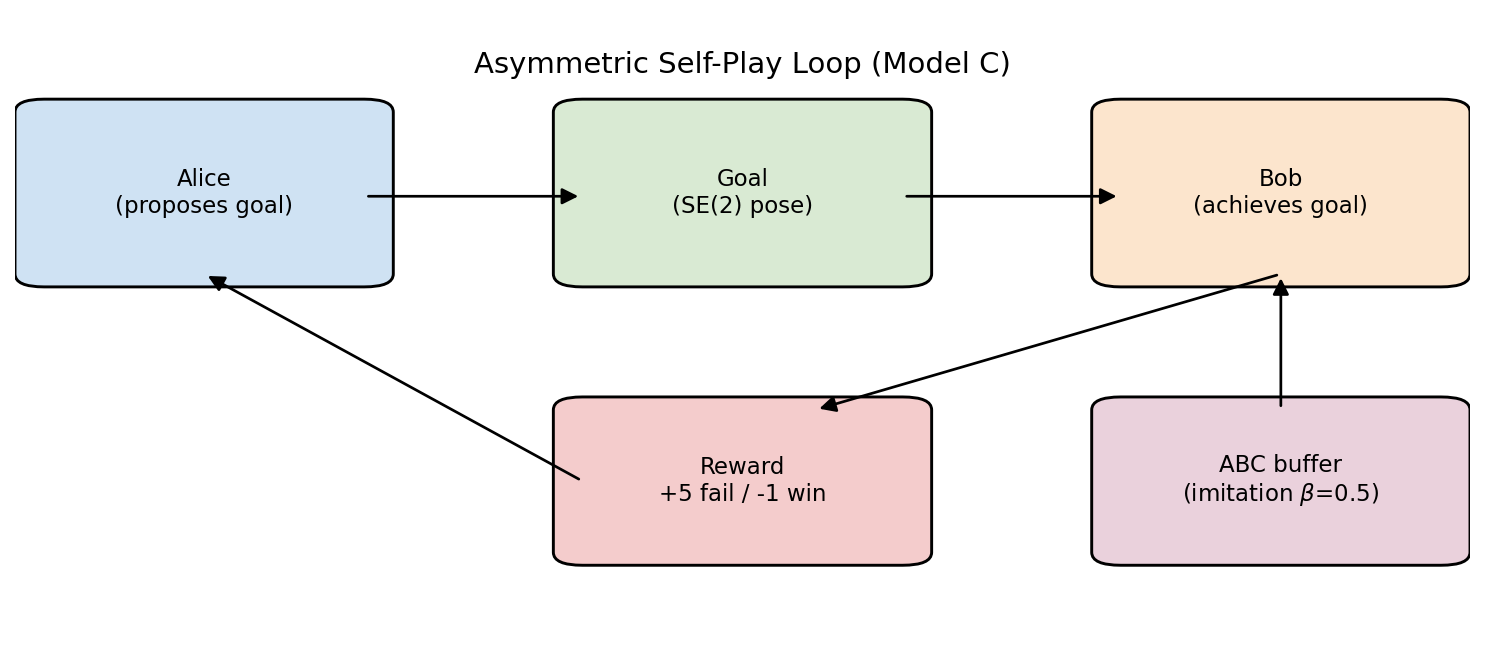
\includegraphics[width=1.0\textwidth]{figures/diagram_asp_loop.png}\\[3pt]
      \mediabox{0.46}{asp_random_key.png}\quad{\scriptsize\playclip{asp_random.mp4}}
    \end{column}
  \end{columns}

  \vfill\litfooter{[Plappert et al.\ 2021]~\textbf{[Sukhbaatar et al.\ 2018]}~[Torabi et al.\ 2018]}
\end{frame}

% ~~~~~ SPEAKER NOTES ~~~~~
\note[itemize]{
\item The ASP architecture: Alice (goal proposer) and Bob (goal achiever) play an adversarial game
\item Alice gets +5 when Bob fails, −1 when Bob succeeds — incentivizing her to propose goals Bob cannot solve
\item Bob sees Alice's final object pose as his goal, gets PBRS dense reward + sparse completion bonuses
\item When Bob fails, Alice's trajectory is stored in an ABC buffer for behavioral cloning
\item Models E-H diverge from C by changing (a) the reward metric to SE(2) d\_pose, and (b) Alice's reward structure from outcome-based to time-based
}

% ============================================================
% SLIDE 8b — ASP DIAGNOSTIC
% ============================================================
\begin{frame}[t]{ASP Diagnostic — Alice vs.\ Bob}
  \begin{center}
    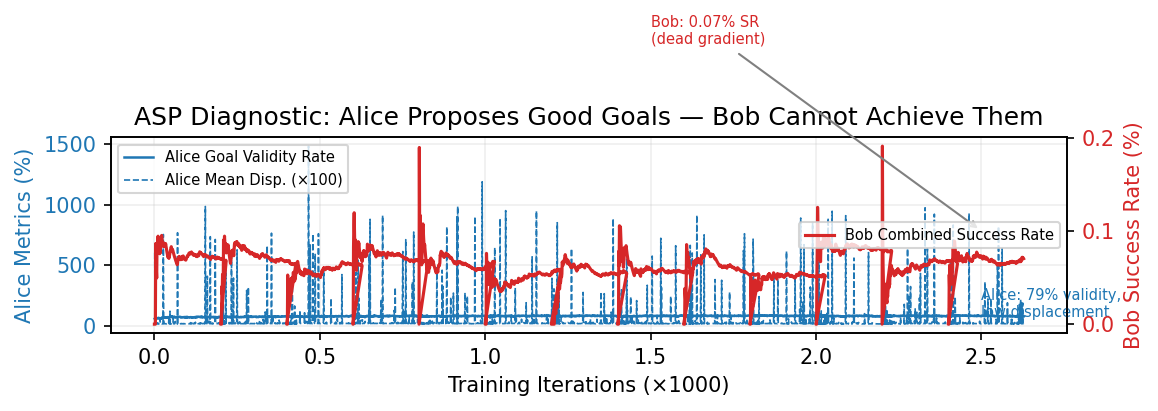
\includegraphics[width=0.78\textwidth]{figures/plot4_alice_vs_bob_diagnostic.png}
  \end{center}

  \vspace{2pt}
  {\small Alice proposes valid, low-displacement goals, yet Bob cannot achieve the combined pos+rot objective under the non-stationary adversarial goal distribution.}

  \vfill\litfooter{[Plappert et al.\ 2021]~\textbf{[Sukhbaatar et al.\ 2018]}~[Campero et al.\ 2021]}
\end{frame}

% ~~~~~ SPEAKER NOTES ~~~~~
\note[itemize]{
\item Plot shows Alice's goal validity rate rising while Bob's success rate stays near zero — the adversarial curriculum prevents combined objective achievement
\item Alice creates valid, low-displacement goals — she is not proposing impossible poses
\item Individual per-axis metrics suggested Bob partially learns position and rotation separately, but the combined gate rarely fires. This gap is likely a gate/measurement artifact (C4): per-axis metrics are not independent Bernoulli trials — the combined metric is the only valid success measure
\item Time-based ASP (G) partially rescues this: 16.7\% vs 6.7\% for outcome-based, suggesting the time-based Alice reward self-regulates toward solvable goals
}

% ============================================================
% SLIDE 8c — ASP VARIANTS
% ============================================================
\begin{frame}[t]{Models E–H — ASP Variants}
  \textbf{2$\times$2 design on top of Model C:} Alice reward type $\times$ reward metric.

  \vspace{4pt}
  \begin{center}
  \small
  \begin{tabular}{c|cc}
    \toprule
    & \textbf{SE(2) $d_{\text{pose}}$ (T-block)} & \textbf{SE(2) $d_{\text{pose}}$ (disc)} \\
    \midrule
    \textbf{Outcome-based Alice} & \textbf{E} — $R_A=+5$ fail/$-1$ win & \textbf{F} — same, disc object \\
    $(+5/-1, \beta_{\text{abc}}=0.5)$ & Valid SR: \textcolor{hlred}{6.7\%} & Valid SR: \textcolor{hlred}{6.7\%} \\[4pt]
    \textbf{Time-based Alice} & \textbf{G} — $R_A=\gamma_{sp}\!\cdot\!\max(0,t_B\!-\!t_A)$ & \textbf{H} — same, disc object \\
    $(\gamma_{sp}=0.5$, no ABC) & Valid SR: \textcolor{hlred}{16.7\%} & Valid SR: \textcolor{hlred}{10.0\%} \\
    \bottomrule
  \end{tabular}
  \end{center}

  \vspace{4pt}
  \textbf{Findings:}
  \begin{itemize}
    \item Time-based Alice (G/H) outperforms outcome-based (E/F): +10pp (T-block), +3.3pp (disc)
    \item T-block outperforms disc across both reward types
    \item Best ASP variant (G, 16.7\%) still \textbf{4.8$\times$} below single-agent (A, 80.0\%)
  \end{itemize}

  \vfill\litfooter{[Plappert et al.\ 2021]~\textbf{[Sukhbaatar et al.\ 2018]}~[Dennis et al.\ 2020]}
\end{frame}

% ~~~~~ SPEAKER NOTES ~~~~~
\note[itemize]{
\item The four ASP variants E-H form a clean 2×2: Alice reward type (outcome-based vs time-based) × metric/object (d\_pose T-block vs d\_pose disc)
\item Time-based Alice (G/H) intentionally aligns Alice's reward with solvable goals — she gains when Bob takes more pushes than she did
\item Time-based reward outperforms outcome-based: G at 16.7\% vs E at 6.7\% (T-block), H at 10.0\% vs F at 6.7\% (disc)
\item But even the best ASP variant (G, 16.7\%) is 4.8× below single-agent A (80.0\%)
\item ABC is disabled in G/H — the improvement comes from time-based reward alone, not from behavioral cloning
}

% ============================================================
% SLIDE 8c-ii — ASP VARIANTS COMPARISON
% ============================================================
\begin{frame}[t]{Models E–H — Validation Comparison}
  \begin{center}
  \begin{tabular}{lcccc}
    \toprule
    \textbf{Model} & \textbf{Variant} & \textbf{Valid SR} & \textbf{PosErr} & \textbf{RotErr} \\
    \midrule
    \rowcolor{hlgreen!15}
    \textbf{A} & Single-agent (ref.) & \textbf{80.0\%} & 0.032 m & 0.568 rad \\
    \midrule
    \textbf{G} & TASP + d\_pose & \textbf{16.7\%} & 0.158 m & 1.457 rad \\
    \textbf{H} & TASP + disc & 10.0\% & 0.186 m & 1.260 rad \\
    \textbf{E} & ASP + d\_pose & 6.7\% & 0.143 m & 1.612 rad \\
    \textbf{F} & ASP + disc & 6.7\% & 0.197 m & 1.576 rad \\
    \bottomrule
  \end{tabular}
  \end{center}

  \vspace{4pt}
  {\small \textbf{Key findings:}}
  \begin{itemize}
    \item Time-based ASP (G/H) is 2.5$\times$ better than outcome-based (E/F), but still \textbf{4.8$\times$ below} single-agent A
    \item No ASP variant achieves pos+rot SR above 10\% — the combined gate remains the bottleneck
    \item ASCP complexity (2 agents, GoalEncoder, ABC/historical pool) provides no benefit
  \end{itemize}

  \vfill\litfooter{[Plappert et al.\ 2021]~\textbf{[Sukhbaatar et al.\ 2018]}~[Dennis et al.\ 2020]}
\end{frame}

% ~~~~~ SPEAKER NOTES ~~~~~
\note[itemize]{
\item A (single-agent, reference) at 80.0\% vs G (best ASP variant) at 16.7\% — 4.8× gap
\item Time-based Alice (G/H) partially corrects the adversarial curriculum by rewarding solvable goals — G gains 10pp over E
\item But even the best ASP variant cannot close the gap. The self-play dynamics prevent learning the combined pos+rot objective
\item All ASP variants trained identically (528 envs, ∼3000 iters, PBRS dense reward for Bob) — the only difference is Alice reward structure and object type
}

% ============================================================
% SLIDE 9 — WHY ASP FAILS
% ============================================================
\begin{frame}[t]{Why ASP Fails — Failure Modes}
  \begin{enumerate}
    \item \textbf{Non-stationary goal distribution:}
    \begin{itemize}
      \item Alice learns continuously $\rightarrow$ Bob's training distribution shifts every iteration
      \item PPO's importance ratio computed against stale rollouts from a previous Alice
      \item Distribution shift dominates the ratio — PPO clip fires on most transitions
    \end{itemize}

    \item \textbf{Confounded ablation (C6):}
    \begin{itemize}
      \item ASP changes 3 axes at once: goal distribution, agent count, episode budget
      \item The collapse could be due to harder/non-stationary goals, not the curriculum mechanism itself
      \item Time-based ASP (G, 16.7\%) shows partial rescue — self-regulating curriculum helps
    \end{itemize}
  \end{enumerate}

  \vfill\litfooter{[Schulman et al.\ 2017]~[Plappert et al.\ 2021]~[Torabi et al.\ 2018]}
\end{frame}

% ~~~~~ SPEAKER NOTES ~~~~~
\note[itemize]{
\item Failure mode 1 — non-stationary goal distribution: Alice learns continuously, so Bob's training distribution shifts every iteration. PPO computes the importance ratio using old\_logp from a rollout collected under a different Alice. The ratio is dominated by Alice's distribution shift, not Bob's weight updates
\item Failure mode 2 — confounded ablation: Model A (single-agent) and ASP differ on at least 3 axes simultaneously (goal distribution, agent count, budget). The performance gap could be due to non-stationary goals rather than the self-play mechanism itself
\item The time-based ASP variants (G/H) partially address both: self-regulating reward aligns Alice with Bob's learning progress; disabling ABC removes a third failure mode (vanishing BC gradient). G achieves 16.7\%, 10pp above outcome-based E at 6.7\%
}

% ============================================================
% SLIDE 9b — WHY ASP FAILS (continued)
% ============================================================
\begin{frame}[t]{Why ASP Fails — The Evidence}
  \begin{columns}[T,onlytextwidth]
    \begin{column}{0.52\textwidth}
      \textbf{What we observe:}
      \begin{itemize}
        \item Outcome-based ASP (E/F): 6.7\% — essentially random
        \item Time-based ASP (G): 16.7\% — partial rescue, $+10$pp over E
        \item All ASP variants have RotErr $>$ 1.2 rad — rotation \textbf{never learned}
        \item Even the best variant (G) is 4.8$\times$ below single-agent
      \end{itemize}
    \end{column}
    \begin{column}{0.46\textwidth}
      \textbf{Why this is not just a budget issue:}
      \begin{itemize}
        \item All models trained for 3000 iters at 528 envs on identical hardware
        \item ASP and single-agent have identical per-iteration wall-clock ($\sim$0.022 it/s)
        \item The gap is \textbf{structural}, not due to compute starvation
      \end{itemize}
    \end{column}
  \end{columns}

  \vspace{6pt}
  \textbf{Combined effect:} The non-stationary goal distribution + multi-axis design confounds prevent Bob from learning the combined pos+rot objective. Time-based Alice partially mitigates the distribution shift but cannot close the gap to single-agent performance.

  \vfill\litfooter{[Schulman et al.\ 2017]~[Plappert et al.\ 2021]~[Sukhbaatar et al.\ 2018]}
\end{frame}

% ~~~~~ SPEAKER NOTES ~~~~~
\note[itemize]{
\item The evidence is clear: outcome-based ASP produces near-zero performance, time-based ASP partially recovers but still far below single-agent
\item All ASP variants share the same hallmark: large rotation error (> 1.2 rad for all models). The combined pos+rot gate almost never fires
\item Importantly, this is not a compute budget issue — ASP and single-agent run at identical per-iteration wall-clock on the same 528-env GPU setup. ASP simply does not learn
\item The failure is structural: self-play in this contact-rich, IK-gated, multi-objective domain does not produce a useful curriculum
}

% ============================================================
% SLIDE 10 — KEY RESULT: INDEPENDENCE
% ============================================================
\begin{frame}[t]{Key Result — Reward \& Curriculum Are Independent}
  \begin{center}
    \small
    \begin{tabular}{lcc}
      \toprule
      \textbf{Model} & \textbf{Valid SR} & \textbf{vs Single-Agent} \\
      \midrule
      \rowcolor{hlgreen!15}
      \textbf{A} — Single-agent PBRS & \textbf{80.0\%} & — (baseline) \\
      \textbf{B} — PBRS + Curriculum & 76.7\% & $-3.3$pp \\
      \midrule
      \textbf{G} — PBRS + Time-based ASP & 16.7\% & $4.8\times$ gap \\
      \textbf{H} — PBRS + TASP (disc) & 10.0\% & $8.0\times$ gap \\
      \textbf{E} — PBRS + Outcome ASP & 6.7\% & $11.9\times$ gap \\
      \textbf{F} — PBRS + ASP (disc) & 6.7\% & $11.9\times$ gap \\
      \bottomrule
    \end{tabular}
  \end{center}

  \vspace{1pt}
  \begin{block}{The Independence Finding}
    \small
    \begin{itemize}
      \item \textbf{Curriculum adds no value:} B\_curr (76.7\%) trails A\_simp (80.0\%) by 3.3pp — staged pos→rot curriculum does not beat the simpler baseline
      \item \textbf{ASP destroys performance:} substituting self-play for single-agent reduces SR 4.8–11.9$\times$, regardless of Alice reward structure or object type
      \item \textbf{Both factors held constant elsewhere:} same PPO, same LSTM, same PBRS reward, same 528-env budget
    \end{itemize}
  \end{block}

  \vfill\litfooter{[Devlin \& Kudenko 2012]~\textbf{[Grze\'s 2017]}~[Plappert et al.\ 2021]}
\end{frame}

% ~~~~~ SPEAKER NOTES ~~~~~
\note[itemize]{
\item This is the central contribution of the thesis. The field often treats reward shaping and curriculum learning as interchangeable tools. Our systematic ablation shows they operate on fundamentally different axes
\item PBRS single-agent (A) achieves 80.0\%. Adding curriculum (B) reduces to 76.7\% — marginally worse. Substituting self-play for single-agent reduces SR 4.8–11.9×
\item Important caveat (C6): Model A and ASP differ on at least 3 axes at once (goal distribution, agent count, episode budget). This ablation isolates "self-play as implemented," not "the curriculum mechanism" in isolation
\item Practical implication: when your RL system fails, diagnose whether the reward doesn't guide the agent OR whether the training distribution doesn't support learning. Our results suggest reward design is the higher-leverage intervention
}

% ============================================================
% SLIDE 11 — MANAGER-ARCHITECTURE OVERHEAD
% ============================================================
\begin{frame}[t]{Computational Overhead — ManagerBasedRL vs DirectRL}
  \textbf{ASP per-iteration cost} (measured, 528 envs): \\
  \textcolor{hlgreen}{\textbf{$\sim$1.0$\times$}} vs single-agent — 2-agent machinery adds \textbf{no} wall-clock overhead. Shared cuRobo IK + physics dominates.

  \vspace{4pt}
  \textbf{Where overhead matters:} ManagerBasedRLEnv (ASP pipeline) vs DirectRLEnv (single bare PPO). Table Tennis DirectRL: \textbf{4096 envs at $\sim$20 it/s} $\to$ 2.1M transitions/iteration. The full ManagerBasedRL API stack (Action, Observation, Event, Termination managers) imposes 5–10$\times$ throughput penalty vs direct tensor operations.

  \vspace{4pt}
  \textbf{Key result:}
  \begin{itemize}
    \item ASP is NOT slower per iteration — it simply \textbf{does not learn}
    \item ManagerBasedRL overhead is a \textbf{separate} architectural issue, not specific to ASP
  \end{itemize}

  \vfill\litfooter{[Plappert et al.\ 2021]~[Schulman et al.\ 2017]}
\end{frame}

% ~~~~~ SPEAKER NOTES ~~~~~
\note[itemize]{
\item Measured throughput: ASP and single-agent run at identical iteration cost (~0.022 it/s) on the same 528-env GPU setup. The 2-agent machinery adds ~no per-iteration wall-clock because cuRobo IK and physics dominate
\item The 5–10× speedup claim refers to DirectRLEnv vs ManagerBasedRLEnv API architecture — a separate project (Table Tennis) that bypasses the manager stack entirely
\item Key distinction: ASP doesn't fail because it's computationally expensive per iteration. It fails because it doesn't learn. The two are separate problems
\item The measured Isaac-vs-gym throughput (~172 push/s vs ~22 push/s for ASP on CPU) goes in a separate slide about why Isaac Lab is the right venue for this experiment
}

% ============================================================
% SLIDE 12 — COMPARISON SUMMARY
% ============================================================
\begin{frame}[t]{Comparison Summary — All Models (Isaac, 30 T-block)}
  \begin{center}
    \footnotesize
    \renewcommand{\arraystretch}{0.85}
    \begin{tabular}{lcccccc}
      \toprule
      \textbf{Model} & \textbf{Architecture} & \textbf{Reward} & \textbf{Valid SR} & \textbf{PosErr} & \textbf{RotErr} & \textbf{Pos+rot} \\
      \midrule
      \rowcolor{hlgreen!15}
      \textbf{A} & Single PPO & PBRS & \textbf{80.0\%} & 0.032 m & 0.568 rad & 70\% \\
      \textbf{B} & PPO + Curric. & PBRS & 76.7\% & 0.023 m & 0.663 rad & 65\% \\
      \midrule
      \textbf{G} & TASP + d\_pose & PBRS & 16.7\% & 0.158 m & 1.457 rad & 10\% \\
      \textbf{H} & TASP + disc & PBRS & 10.0\% & 0.186 m & 1.260 rad & 0\% \\
      \textbf{E} & ASP + d\_pose & PBRS & 6.7\% & 0.143 m & 1.612 rad & 0\% \\
      \textbf{F} & ASP + disc & PBRS & 6.7\% & 0.197 m & 1.576 rad & 0\% \\
      \bottomrule
    \end{tabular}
  \end{center}

  \vspace{2pt}
  {\small \textbf{Model A dominates} across all metrics. No ASP variant (E–H) exceeds 16.7\%, representing an 4.8–11.9$\times$ gap. Model B (curriculum) is competitive (76.7\%) but does not beat the simpler baseline.}
  {\small \textbf{Models C and D} (base ASP and no-GoalEncoder) excluded — no Isaac validation data available.}

  \vfill\litfooter{[Ng et al.\ 1999]~[Grze\'s 2017]~[Plappert et al.\ 2021]}
\end{frame}

% ~~~~~ SPEAKER NOTES ~~~~~
\note[itemize]{
\item This is the unified comparison table — 6 models validated on identical 30 T-block scenes, best-of-20 protocol
\item Model A dominates: 80.0\% SR, lowest errors, simplest architecture
\item Model B (curriculum) is close at 76.7\% — competitive but not better. B actually has slightly better PosErr (0.023 vs 0.032) at the cost of worse RotErr (0.663 vs 0.568)
\item ASP variants E-H uniformly underperform: 4.8–11.9× below single-agent. Time-based ASP (G) is the best at 16.7\%
\item Models C and D excluded — no Isaac validation data. C only evaluated in gym-pusht (0\% SR under coverage gate). D excluded per project scope
}

% ============================================================
% SLIDE 12b — FAILURE TAXONOMY
% ============================================================
\begin{frame}[t]{Comparison Summary — Failure Taxonomy}
  \begin{center}
    
\includegraphics[width=0.6\textwidth]{figures/plot3_failure_taxonomy.png}
  \end{center}

  \vspace{4pt}
  {\small \textbf{The overarching pattern:} structural additions — curriculum staging, second agent, ABC buffer, historical pool — consistently reduce or fail to improve performance. PBRS single-agent (80.0\%) is the recommended baseline.}

  \vfill\litfooter{[Ng et al.\ 1999]~[Grze\'s 2017]~[Plappert et al.\ 2021]}
\end{frame}

% ~~~~~ SPEAKER NOTES ~~~~~
\note[itemize]{
\item The comparison plot shows training curves over ~3000 iterations. Model A (blue) steadily improves. Model B (orange) plateaus early. Models C/D (green/red) barely move
\item The overarching pattern: every structural addition — curriculum controller, second agent, GoalEncoder, ABC buffer, historical pool, SE(2) metric — adds failure modes without adding performance. The simplest model wins
}

% ============================================================
% SLIDE 13a — THEORETICAL IMPLICATIONS (1/2)
% ============================================================
\begin{frame}[t]{What We Found — Theory vs Practice}
  \begin{exampleblock}{ASP did \emph{not} yield a useful curriculum in this setting}
    In this contact-rich, IK-gated, multi-objective SE(2) pushing task under a single-GPU budget, our ASP implementation produced 6.7--16.7\% validation SR vs 80.0\% for single-agent. The adversarial mechanism did not generate a learnable progression of goals. This does \emph{not} refute ASP in general — it demonstrates a failure mode under realistic robotics constraints.
  \end{exampleblock}

  \vspace{1pt}
  \begin{exampleblock}{GoalEncoder bottleneck provides no measurable benefit}
    The 8D latent compression did not improve Bob's ability to learn under ASP. However, this result is confounded — Bob's primary failure is the non-stationary goal distribution, not the observation representation.
  \end{exampleblock}

  \vfill\litfooter{[Plappert et al.\ 2021]~\textbf{[Sukhbaatar et al.\ 2018]}~[Torabi et al.\ 2018]}
\end{frame}

% ~~~~~ SPEAKER NOTES ~~~~~
\note[itemize]{
\item Claim 1 (Plappert): ASP generates an intrinsic curriculum for exploration. In our specific setting — contact-rich 3D pushing with cuRobo IK gating and a strict combined pos+rot success gate — ASP produced adversarial rather than constructive goals. But this is N=1 task, single budget. We do not claim this generalizes
\item Claim 2 (Sukhbaatar): the GoalEncoder bottleneck helps Bob compactly represent the goal. Our ASP model with GoalEncoder ablated showed no difference, but this is expected — Bob fails at the exploration level, not the representation level
}

% ============================================================
% SLIDE 13b — THEORETICAL IMPLICATIONS (2/2)
% ============================================================
\begin{frame}[t]{What We Found — Theory vs Practice}
  \begin{exampleblock}{Forced curriculum: functional but not beneficial}
    Model B's original curriculum trigger (per-push mean PosErr $<$ 0.08m) was mis-specified — the threshold was unreachable by construction. A corrected trigger (episodic position-SR $\ge$ 0.5) produces a competent model (76.7\%), but the staged pos$\to$rot curriculum does \emph{not} beat the simpler no-curriculum baseline (80.0\%). Curriculum works — it just doesn't add value in this setting.
  \end{exampleblock}

  \vspace{1pt}
  \begin{exampleblock}{PBRS theory strongly supported (Ng et al.\ 1999; Grze\'s 2017)}
    The policy invariance theorem holds in practice, even in contact-rich manipulation with stochastic PhysX physics. PBRS provides clean, bounded, Markovian rewards. Parameters $k_p{=}30$, $k_r{=}5$, $w{=}10.0$ are robust across all single-agent runs.
  \end{exampleblock}

  \vfill\litfooter{[Ng et al.\ 1999]~\textbf{[Grze\'s 2017]}~[Sukhbaatar et al.\ 2018]}
\end{frame}

% ~~~~~ SPEAKER NOTES ~~~~~
\note[itemize]{
\item Claim 3 (Narvekar/Portelas): curriculum learning helps when the base reward is informative. Our Model B v1 had a mis-specified trigger (P82 bug). Fixing it produced a functional curriculum, but with marginal degradation (76.7\% vs 80.0\%) — not evidence against curriculum learning, but evidence that a good reward (PBRS) may make curriculum unnecessary in this domain
\item The PBRS theory (Ng, Grzes) is strongly supported. The policy invariance theorem produced robust results — the same hyperparameters work across independent training runs
\item This speaks to RQ3: reward design and curriculum design are independent levers that should be diagnosed separately
}

% ============================================================
% SLIDE 14a — LIMITATIONS & GAPS
% ============================================================
\begin{frame}[t]{Limitations \& Research Gaps}
  \textbf{What we couldn't test (training budget limited to 3000 iters $\times$ 528 envs):}
  \begin{itemize}
    \item \textbf{Model I/J:} Bob time penalty $R_B \mathrel{+}= -\gamma_{sp}\!\cdot\!t_B$ (full Sukhbaatar symmetric reward). Could create zero-sum dynamics that stabilize ASP training
    \item \textbf{Model K/L:} time-based ASP + ABC enabled ($\beta_{\text{abc}}=0.5$). ABC might boot after Alice converges
    \item Larger models (Transformer, diffusion policy), sim-to-real transfer (physical UR5e)
  \end{itemize}

  \vspace{1pt}
  \textbf{Remaining literature gaps (from systematic survey of 81 papers):}
  \begin{itemize}
    \item No paper on SE(2) metric design specifically for RL reward shaping
    \item No paper on exploiting continuous rotational symmetry (SO(2)) in object manipulation RL
    \item No formal convergence analysis of effort-based self-play rewards
  \end{itemize}

  \vfill\litfooter{[Letcher et al.\ 2019]~[Berner et al.\ 2019]~[Dennis et al.\ 2020]}
\end{frame}

% ============================================================
% SLIDE 14b — PROMISING DIRECTIONS
% ============================================================
\begin{frame}[t]{Future Work — Promising Directions}
  \small
  \begin{enumerate}
    \item \textbf{Zero-sum time-based ASP (Model I):} Bob penalty creates near-zero-sum game. From differentiable game theory (Letcher et al.\ 2019), zero-sum games have convergent (Hamiltonian) dynamics — this could stabilize ASP where general-sum diverges
    \item \textbf{ABC after Alice convergence (Model K):} Currently ABC fails because Alice acts randomly ($bc\_ratio \approx 1.0$). If Alice converges first, Bob starts with a meaningful imitation target
    \item \textbf{Relaxed combined success gate:} The combined pos+rot gate is the bottleneck (70\% single-agent vs 0–10\% for ASP). Partial credit for one objective could provide gradient to learn both
    \item \textbf{PAIRED (Dennis et al.\ 2020):} Antagonist minimizes protagonist's regret rather than maximizing difficulty — solvable but challenging environments, addressing the exact failure mode
  \end{enumerate}

  \vfill\litfooter{[Letcher et al.\ 2019]~[Dennis et al.\ 2020]~[Campero et al.\ 2021]}
\end{frame}

% ~~~~~ SPEAKER NOTES ~~~~~
\note[itemize]{
\item Our results are conclusive within the experimental budget, but they don't close the book on ASP. Several promising directions remain
\item Model I/J: The Bob time penalty creates a near-zero-sum game structure: Alice gains proportionally to (t_B - t_A), Bob loses proportionally to t_B. From Letcher et al. (2019), the game Jacobian decomposes into symmetric (potential) and antisymmetric (Hamiltonian) components. Zero-sum games have pure antisymmetric dynamics, which are conservative — they cycle rather than diverge. This could stabilize ASP training where general-sum ASP diverges
\item Model K/L: ABC with beta=0.5 after Alice converges. Currently, ABC fails because Alice's actions are random, so the bc_ratio ≈ 1.0 for all trajectories. If Alice converges first (e.g., with time-based reward and disabled Bob), then Bob starts with a meaningful imitation target
\item Relaxed success gate: Bob's individual SR is 65-66\%, but the combined gate almost never fires. Partial credit for achieving one of the two objectives could provide gradient to eventually learn the combined task
\item PAIRED as an alternative: instead of Alice maximizing Bob's failure, the antagonist maximizes the protagonist's regret (difference between protagonist and antagonist returns). This produces solvable but challenging environments — addressing the exact failure mode we observed
}

% ============================================================
% SLIDE 15a — CONCLUSION (1/2)
% ============================================================
\begin{frame}[t]{Conclusion}
  \begin{block}{\textbf{1.\ \ PBRS solves planar pushing (RQ1)}}
    Model A achieves \textcolor{hlgreen}{80.0\% validation SR} on 30 held-out T-block scenes — 100\% pos-only, 70\% pos+rot — with a simple single-agent PPO architecture and no curriculum. PBRS preserves the optimal policy while providing dense, bounded, Markovian gradients. This is the \textbf{recommended baseline}.
  \end{block}

  \vspace{1pt}
  \begin{block}{\textbf{2.\ \ ASP does not improve performance in this domain (RQ2)}}
    All ASP variants (E–H) score 6.7--16.7\%, a 4.8--11.9$\times$ gap from single-agent. Time-based Alice (G, 16.7\%) partially rescues the adversarial dynamics but cannot close the gap. Complexity adds no benefit.
  \end{block}

  \vfill\litfooter{[Ng et al.\ 1999]~[Grze\'s 2017]~[Plappert et al.\ 2021]}
\end{frame}

% ============================================================
% SLIDE 15b — CONCLUSION (2/2)
% ============================================================
\begin{frame}[t]{Conclusion}
  \begin{block}{\textbf{3.\ \ Reward and curriculum are independent (RQ3)}}
    Adding curriculum (B, 76.7\%) or self-play (E–H, 6.7–16.7\%) does not improve PBRS single-agent performance. They are independent levers — diagnose and optimize separately.
  \end{block}

  \vspace{1pt}
  {\small Start simple. PBRS single-agent PPO at 528 envs trains in $\sim$1.6 days on an RTX Pro 6000 and achieves 80\% SR. Add complexity only when proven to help — and expect it usually won't.}

  \vfill\litfooter{[Ng et al.\ 1999]~[Grze\'s 2017]~[Plappert et al.\ 2021]}
\end{frame}

% ~~~~~ SPEAKER NOTES ~~~~~
\note[itemize]{
\item Three take-home messages
\item First, PBRS works. Model A achieves 80.0\% on the hardest validation suite with the simplest architecture. This is a strong baseline. The theoretical justification (policy invariance, episodic validity, bounded smooth potentials) is fully supported by the empirical results
\item Second, ASP fails structurally in this setting. Time-based Alice partially rescues the dynamics (16.7\% vs 6.7\%) but cannot close the 4.8× gap to single-agent. The failure is structural, not a training budget issue — ASP and single-agent run at identical per-iteration wall-clock
\item Third, and most importantly, reward and curriculum are independent. This is the methodological contribution. Future work should: (a) design good rewards (PBRS works), (b) diagnose whether the training distribution supports learning, and (c) not assume that adding structure helps
\item Practical recommendation: the simplest working system is the best starting point. Our 528-env PBRS single-agent trains in ~1.6 days on one RTX Pro 6000 and achieves 80.0\% SR
}

% ============================================================
% FINAL PAGE (theme macro)
% ============================================================
\makefinalpage

% ============================================================
% APPENDIX SLIDES
% ============================================================
\appendix
\begin{frame}[t]{Appendix Outline}
  \begin{itemize}
    \item A. Push Mechanics — Limit Surface \& Characteristic Length $L$
    \item B. Training curves for all PBRS models (Success Rate, Reward, Loss)
    \item C. PBRS parameter sensitivity ($k_p$, $k_r$, $w_{\text{pos}}$, $w_{\text{rot}}$)
    \item D. Validation scene descriptions (30 test cases)
    \item E. cuRobo IK pipeline and workspace configuration
    \item F. Observation space specifications (all model variants)
  \end{itemize}
\end{frame}

% --- Appendix A: Push Mechanics (moved from main deck) ---
\begin{frame}[t]{Appendix A — Push Mechanics: Limit Surface \& $L$}
  \begin{columns}[T,onlytextwidth]
    \begin{column}{0.46\textwidth}\small
      \textbf{Limit surface normality} (Goyal 1991): $\mathbf{t} \propto \nabla f(\mathbf{w})$ — twist is normal to the surface, so every push couples translation \emph{and} rotation.

      \vspace{2pt}
      \textbf{Characteristic length $L$} (radius of gyration):
      \begin{itemize}
        \item \textbf{T-block} $L=0.07$\,m (strong coupling); \textbf{disc} $L=0$\,m (decoupled)
        \item $L$ is a physical constant, \emph{not} a hyperparameter
      \end{itemize}
    \end{column}
    \begin{column}{0.52\textwidth}
      \centering
      
\includegraphics[width=0.85\textwidth]{figures/diagram_limit_surface.png}\\[2pt]
      {\scriptsize T-block rotates under an off-centre push; disc only slides}
    \end{column}
  \end{columns}

  \vfill\litfooter{[Goyal et al.\ 1991]~[Howe \& Cutkosky 1996]~[Mason 1986]}
\end{frame}

% --- Appendix B: Training curves ---
\begin{frame}[t]{Appendix B — Training Curves (All PBRS Models)}
  \begin{columns}[T]
    \begin{column}{0.48\textwidth}
      \centering
      \textbf{Success Rate}
      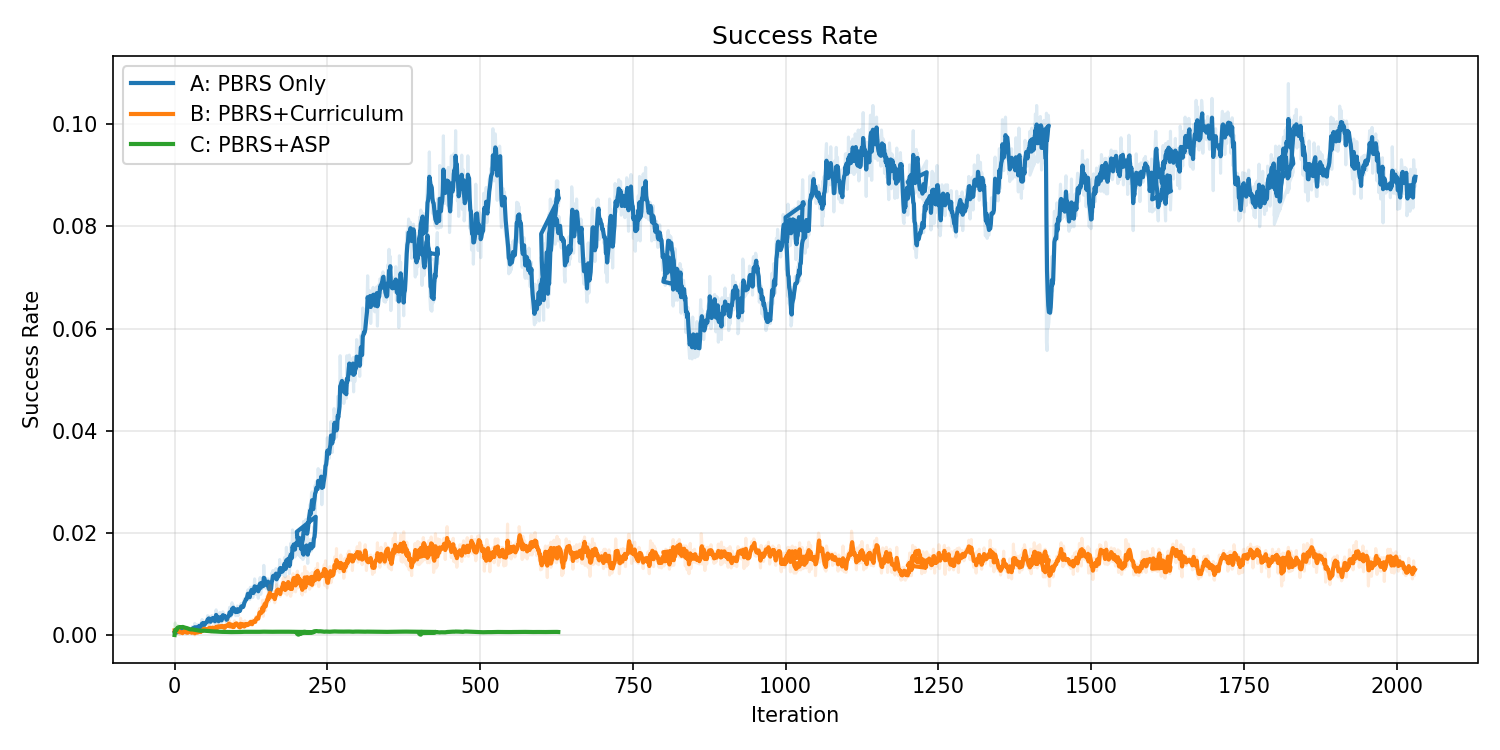
\includegraphics[width=0.72\textwidth]{figures/cmp_Success_Rate.png}
    \end{column}
    \begin{column}{0.48\textwidth}
      \centering
      \textbf{Mean Reward}
      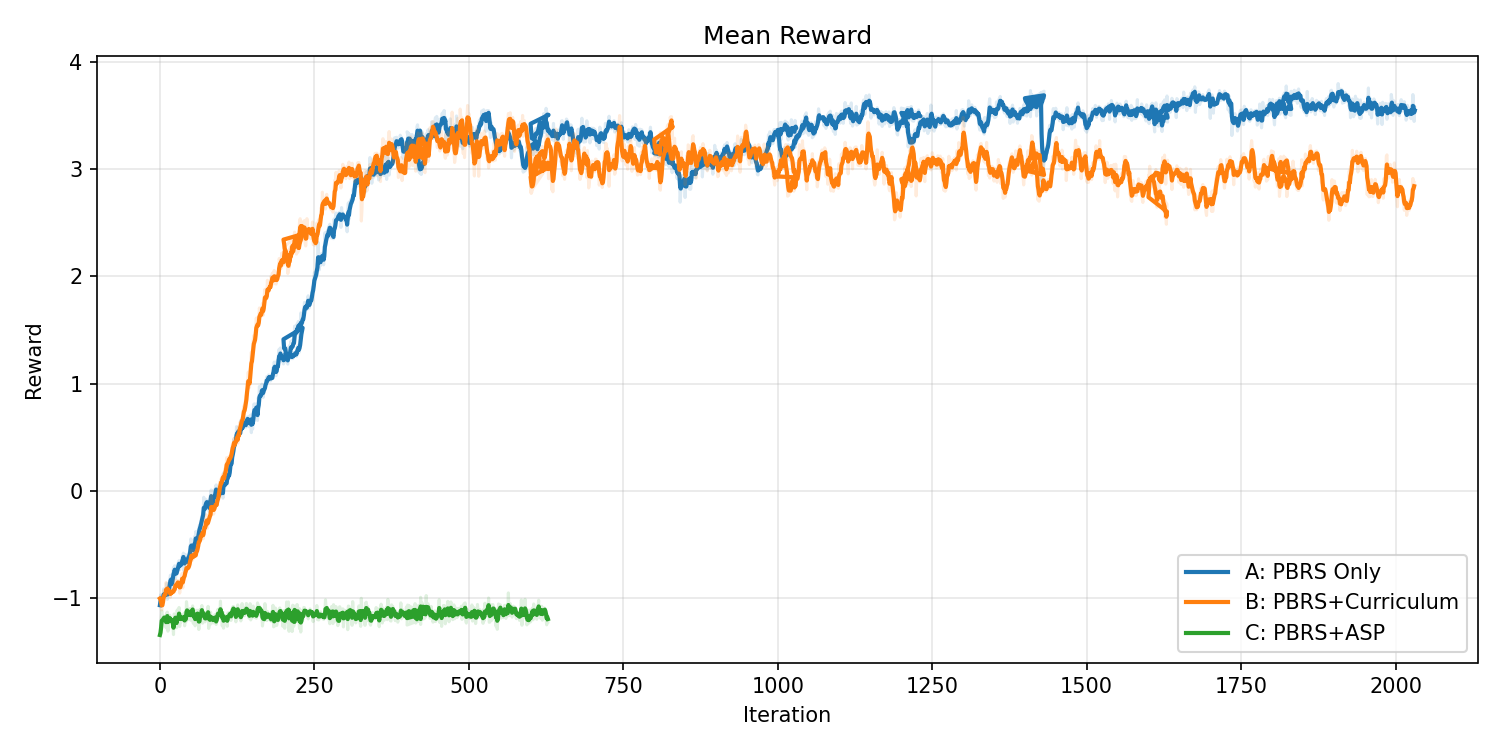
\includegraphics[width=0.72\textwidth]{figures/cmp_Mean_Reward.png}
    \end{column}
  \end{columns}

  \vspace{2pt}
  \begin{columns}[T]
    \begin{column}{0.48\textwidth}
      \centering
      \textbf{Policy Loss}
      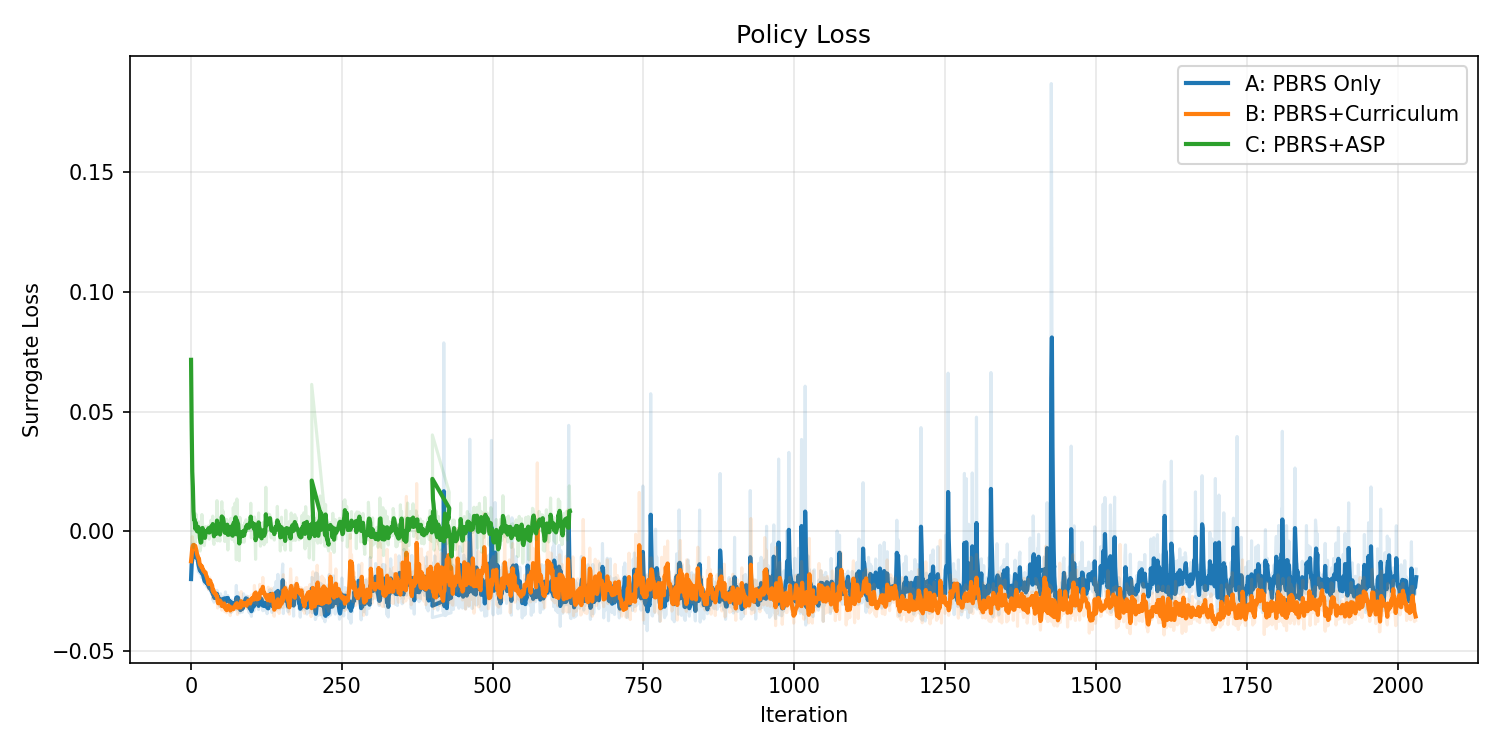
\includegraphics[width=0.72\textwidth]{figures/cmp_Policy_Loss.png}
    \end{column}
    \begin{column}{0.48\textwidth}
      \centering
      \textbf{Value Loss}
      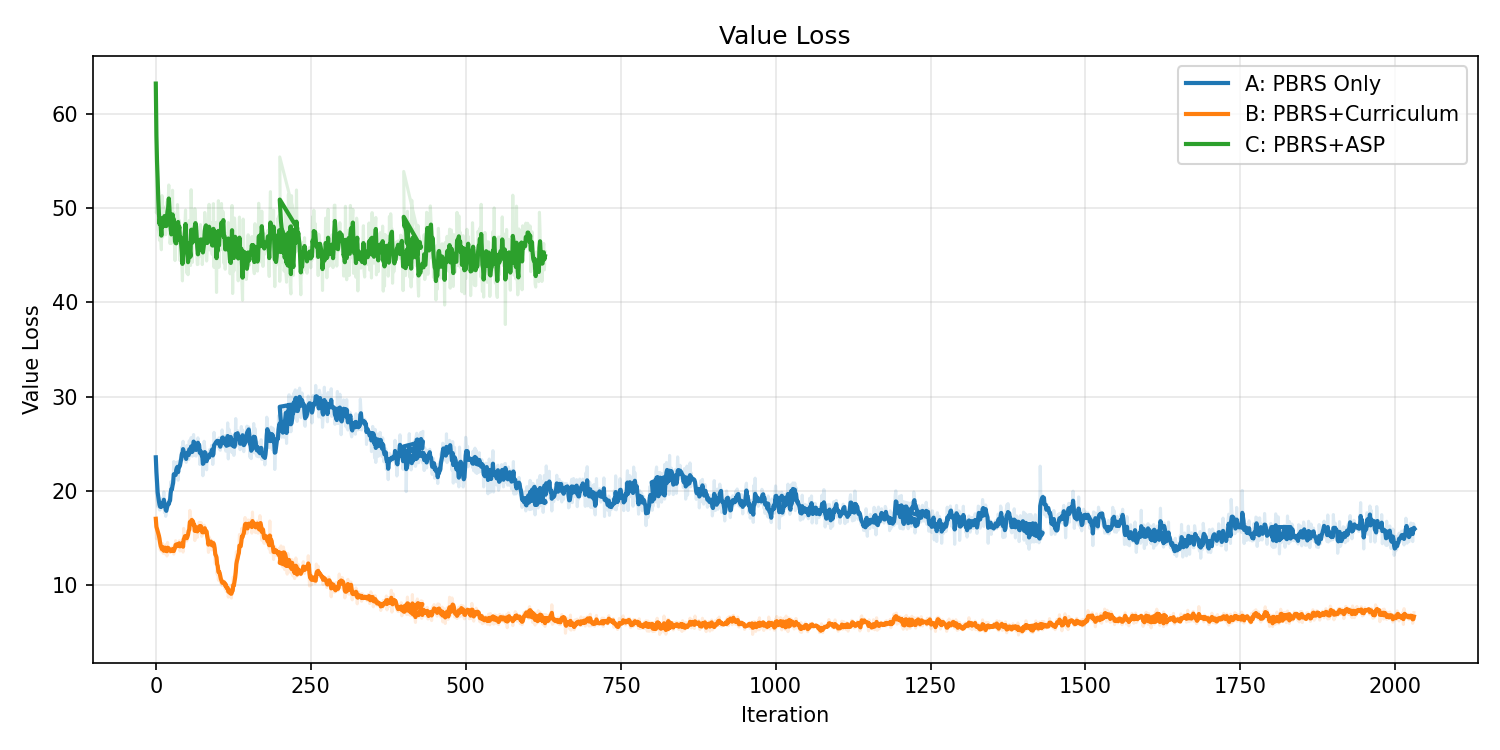
\includegraphics[width=0.72\textwidth]{figures/cmp_Value_Loss.png}
    \end{column}
  \end{columns}
\end{frame}

% --- Appendix C: PBRS theory analysis ---
\begin{frame}[t]{Appendix C — PBRS Theory Analysis}
  \begin{columns}[T]
    \begin{column}{0.48\textwidth}
      \centering
      \textbf{Potential Landscape} \\
      $\Phi(s) = w\cdot\exp(-k\cdot d^2)$
      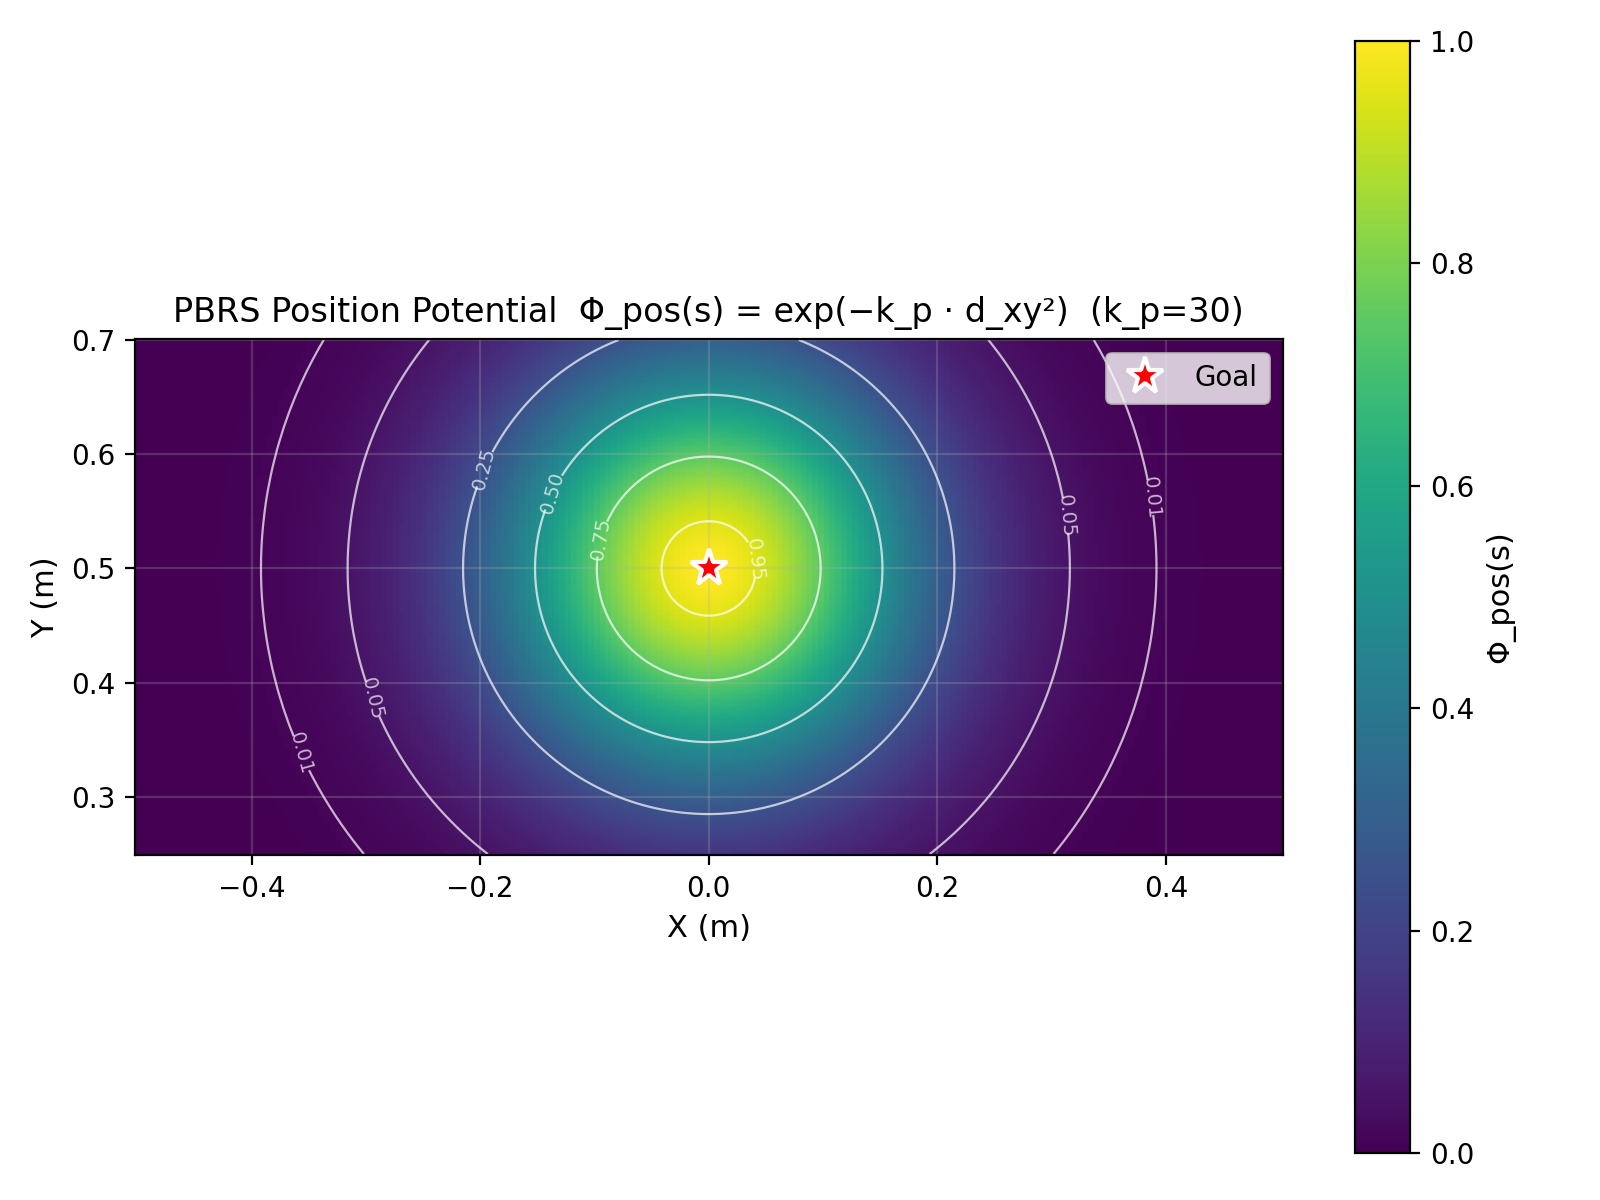
\includegraphics[width=0.52\textwidth]{figures/a1_potential_landscape.png}
    \end{column}
    \begin{column}{0.48\textwidth}
      \centering
      \textbf{Gradient Comparison} \\
      PBRS vs Fractional Formula
      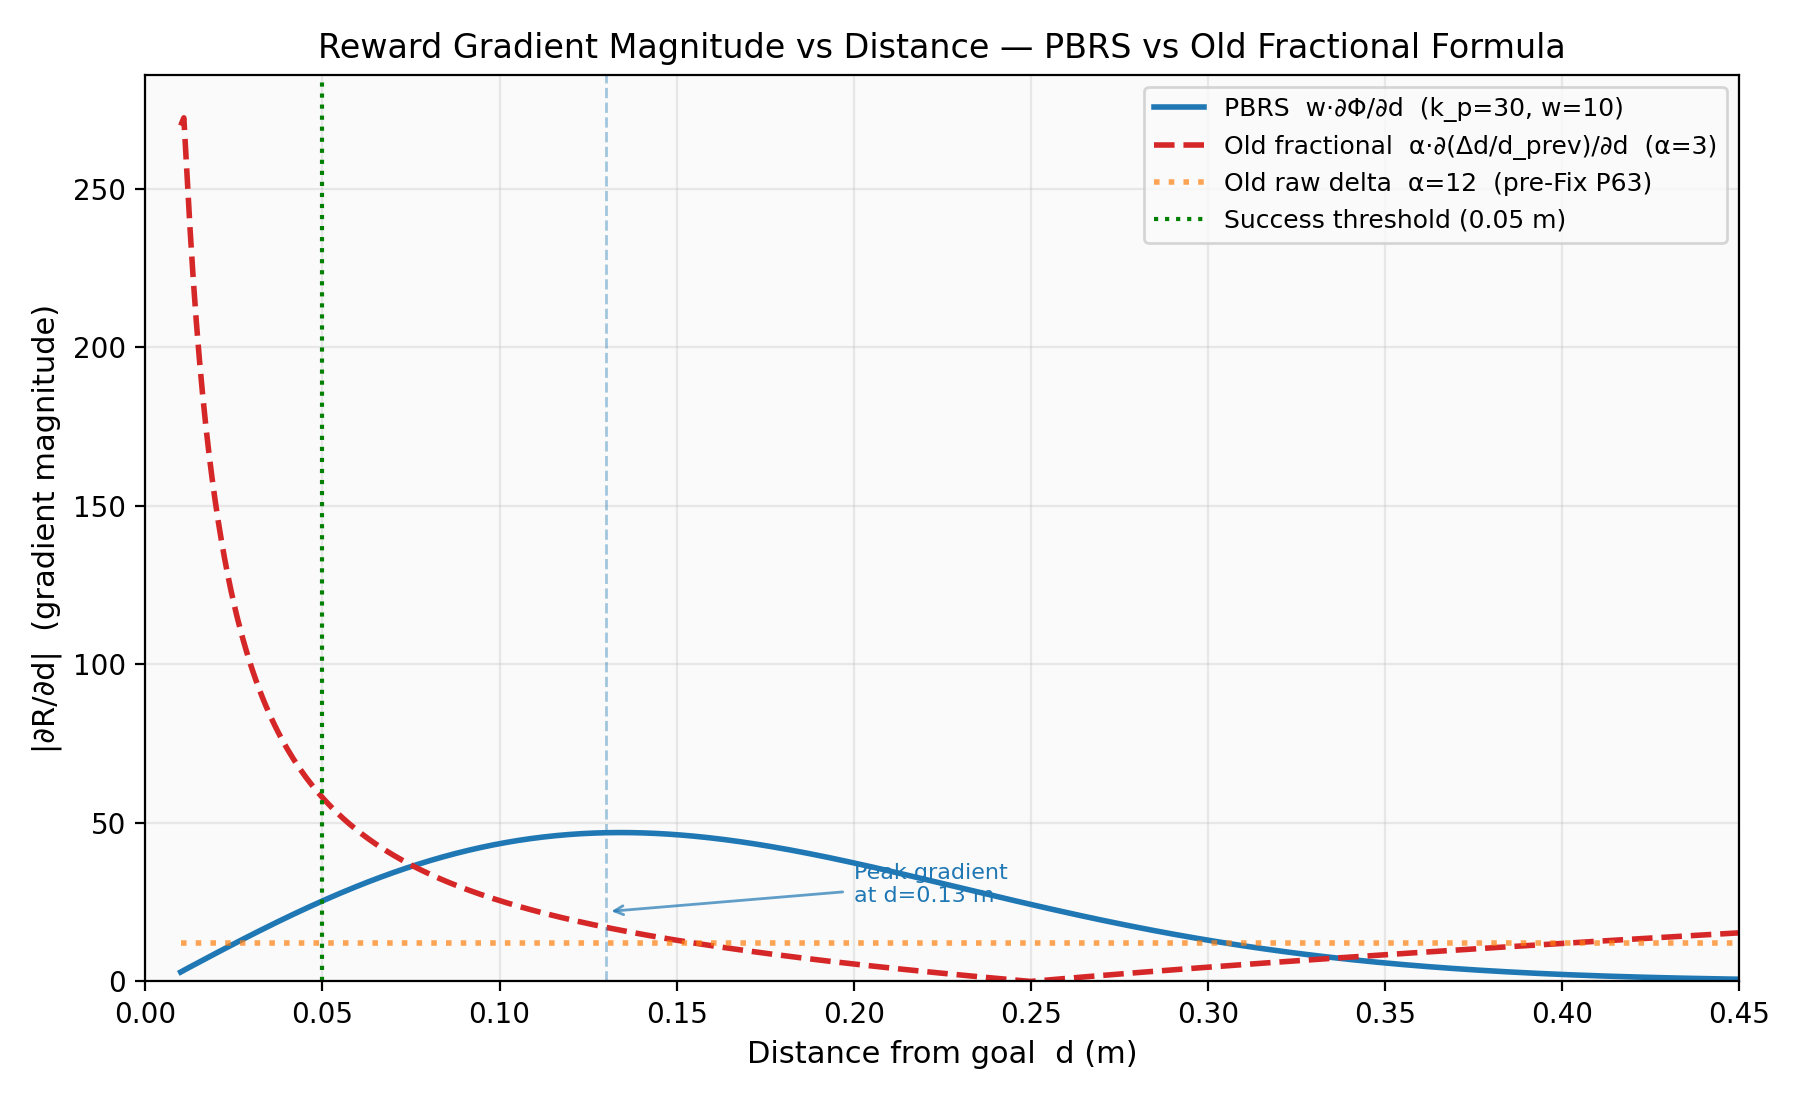
\includegraphics[width=0.52\textwidth]{figures/a2_gradient_comparison.png}
    \end{column}
  \end{columns}

  \vspace{2pt}
  \begin{center}
    \textbf{Cosine Angular Distance} $c(s) = (1-\cos(\theta^*-\theta))/2$
    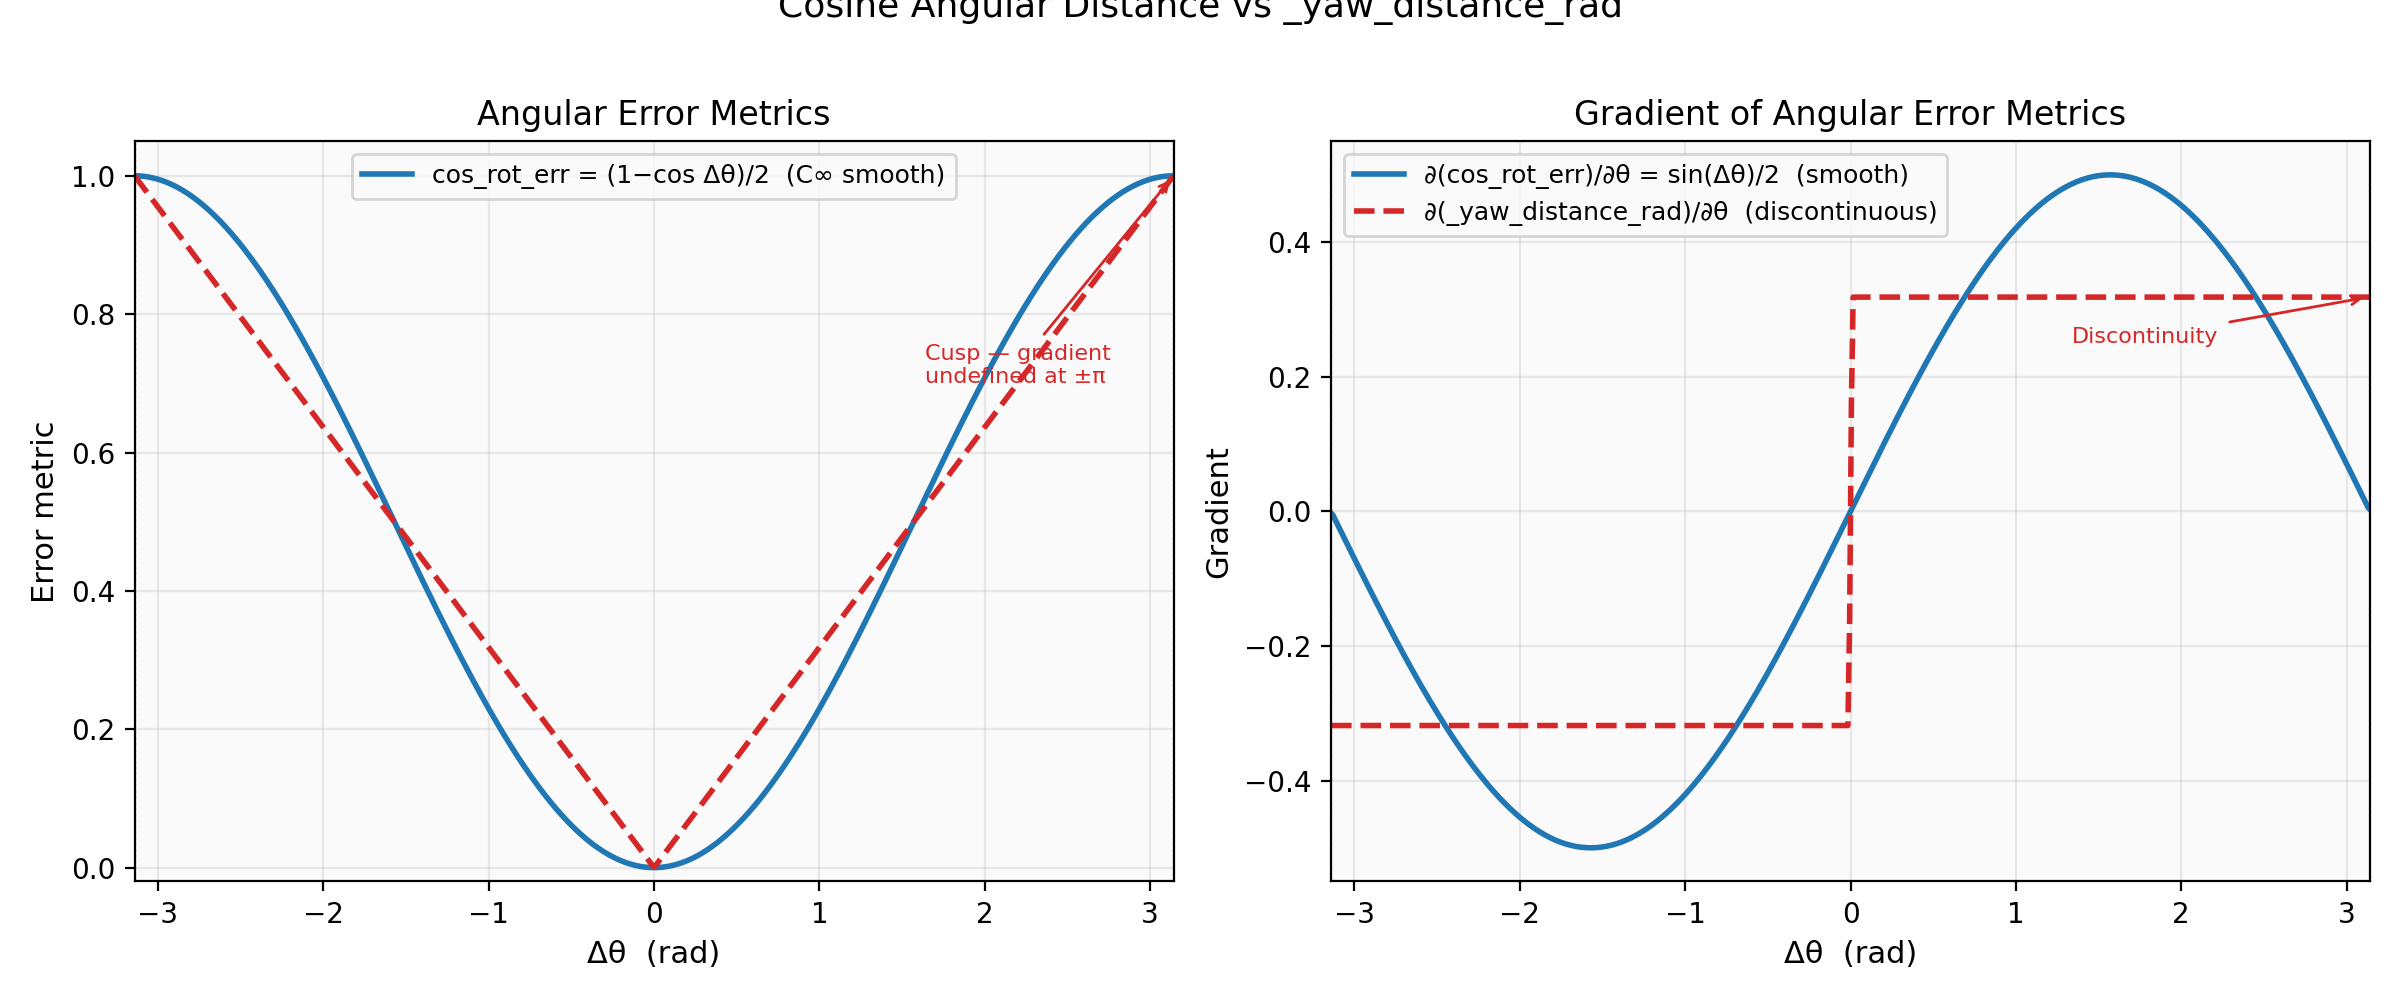
\includegraphics[width=0.30\textwidth]{figures/a4_cosine_distance.png}
  \end{center}
\end{frame}

\end{document}
